% Created 2020-08-26 qua 20:37
% Intended LaTeX compiler: pdflatex
\documentclass[11pt]{article}
\usepackage[utf8]{inputenc}
\usepackage{lmodern}
\usepackage[T1]{fontenc}
\usepackage[top=2cm, bottom=2cm, left=2cm, right=2cm]{geometry}
\usepackage{graphicx}
\usepackage{longtable}
\usepackage{float}
\usepackage{wrapfig}
\usepackage{rotating}
\usepackage[normalem]{ulem}
\usepackage{amsmath}
\usepackage{textcomp}
\usepackage{marvosym}
\usepackage{wasysym}
\usepackage{amssymb}
\usepackage{amsmath}
\usepackage[theorems, skins]{tcolorbox}
\usepackage[style=abnt,noslsn,extrayear,uniquename=init,giveninits,justify,sccite,
scbib,repeattitles,doi=false,isbn=false,url=false,maxcitenames=2,
natbib=true,backend=biber]{biblatex}
\usepackage{url}
\usepackage[linktocpage,pdfstartview=FitH,colorlinks,
linkcolor=blue,anchorcolor=blue,
citecolor=blue,filecolor=blue,menucolor=blue,urlcolor=blue]{hyperref}
\usepackage{attachfile}
\usepackage{setspace}
\usepackage{tikz}
\author{Pedro Paulo Zahluth Bastos, Luiz Celso Gomes Jr, Lorena Salces Dourado, Gabriel Petrini, Paulo Robilloti, Antonio Ibarra}
\date{September 2020}
\title{Impactos econômicos da COVID-19}
\begin{document}

\maketitle
\tableofcontents


\section{Dados Granulares}
\label{sec:org8501ce0}

\subsection{Energia}
\label{sec:org6aa200b}

\emph{home/gpetrini}.local/lib/python3.8/site-packages/pandas\_datareader/compat/\_\_init\_\_.py:7: FutureWarning: pandas.util.testing is deprecated. Use the functions in the public API at pandas.testing instead.
  from pandas.util.testing import assert\_frame\_equal


\subsubsection{Brazil: BRA}
\label{sec:org5a9297e}
\begin{enumerate}
\item Energy share
\label{sec:org5c8cb00}

\begin{verbatim}
<Figure size 2400x1500 with 1 Axes>
\end{verbatim}


\begin{center}
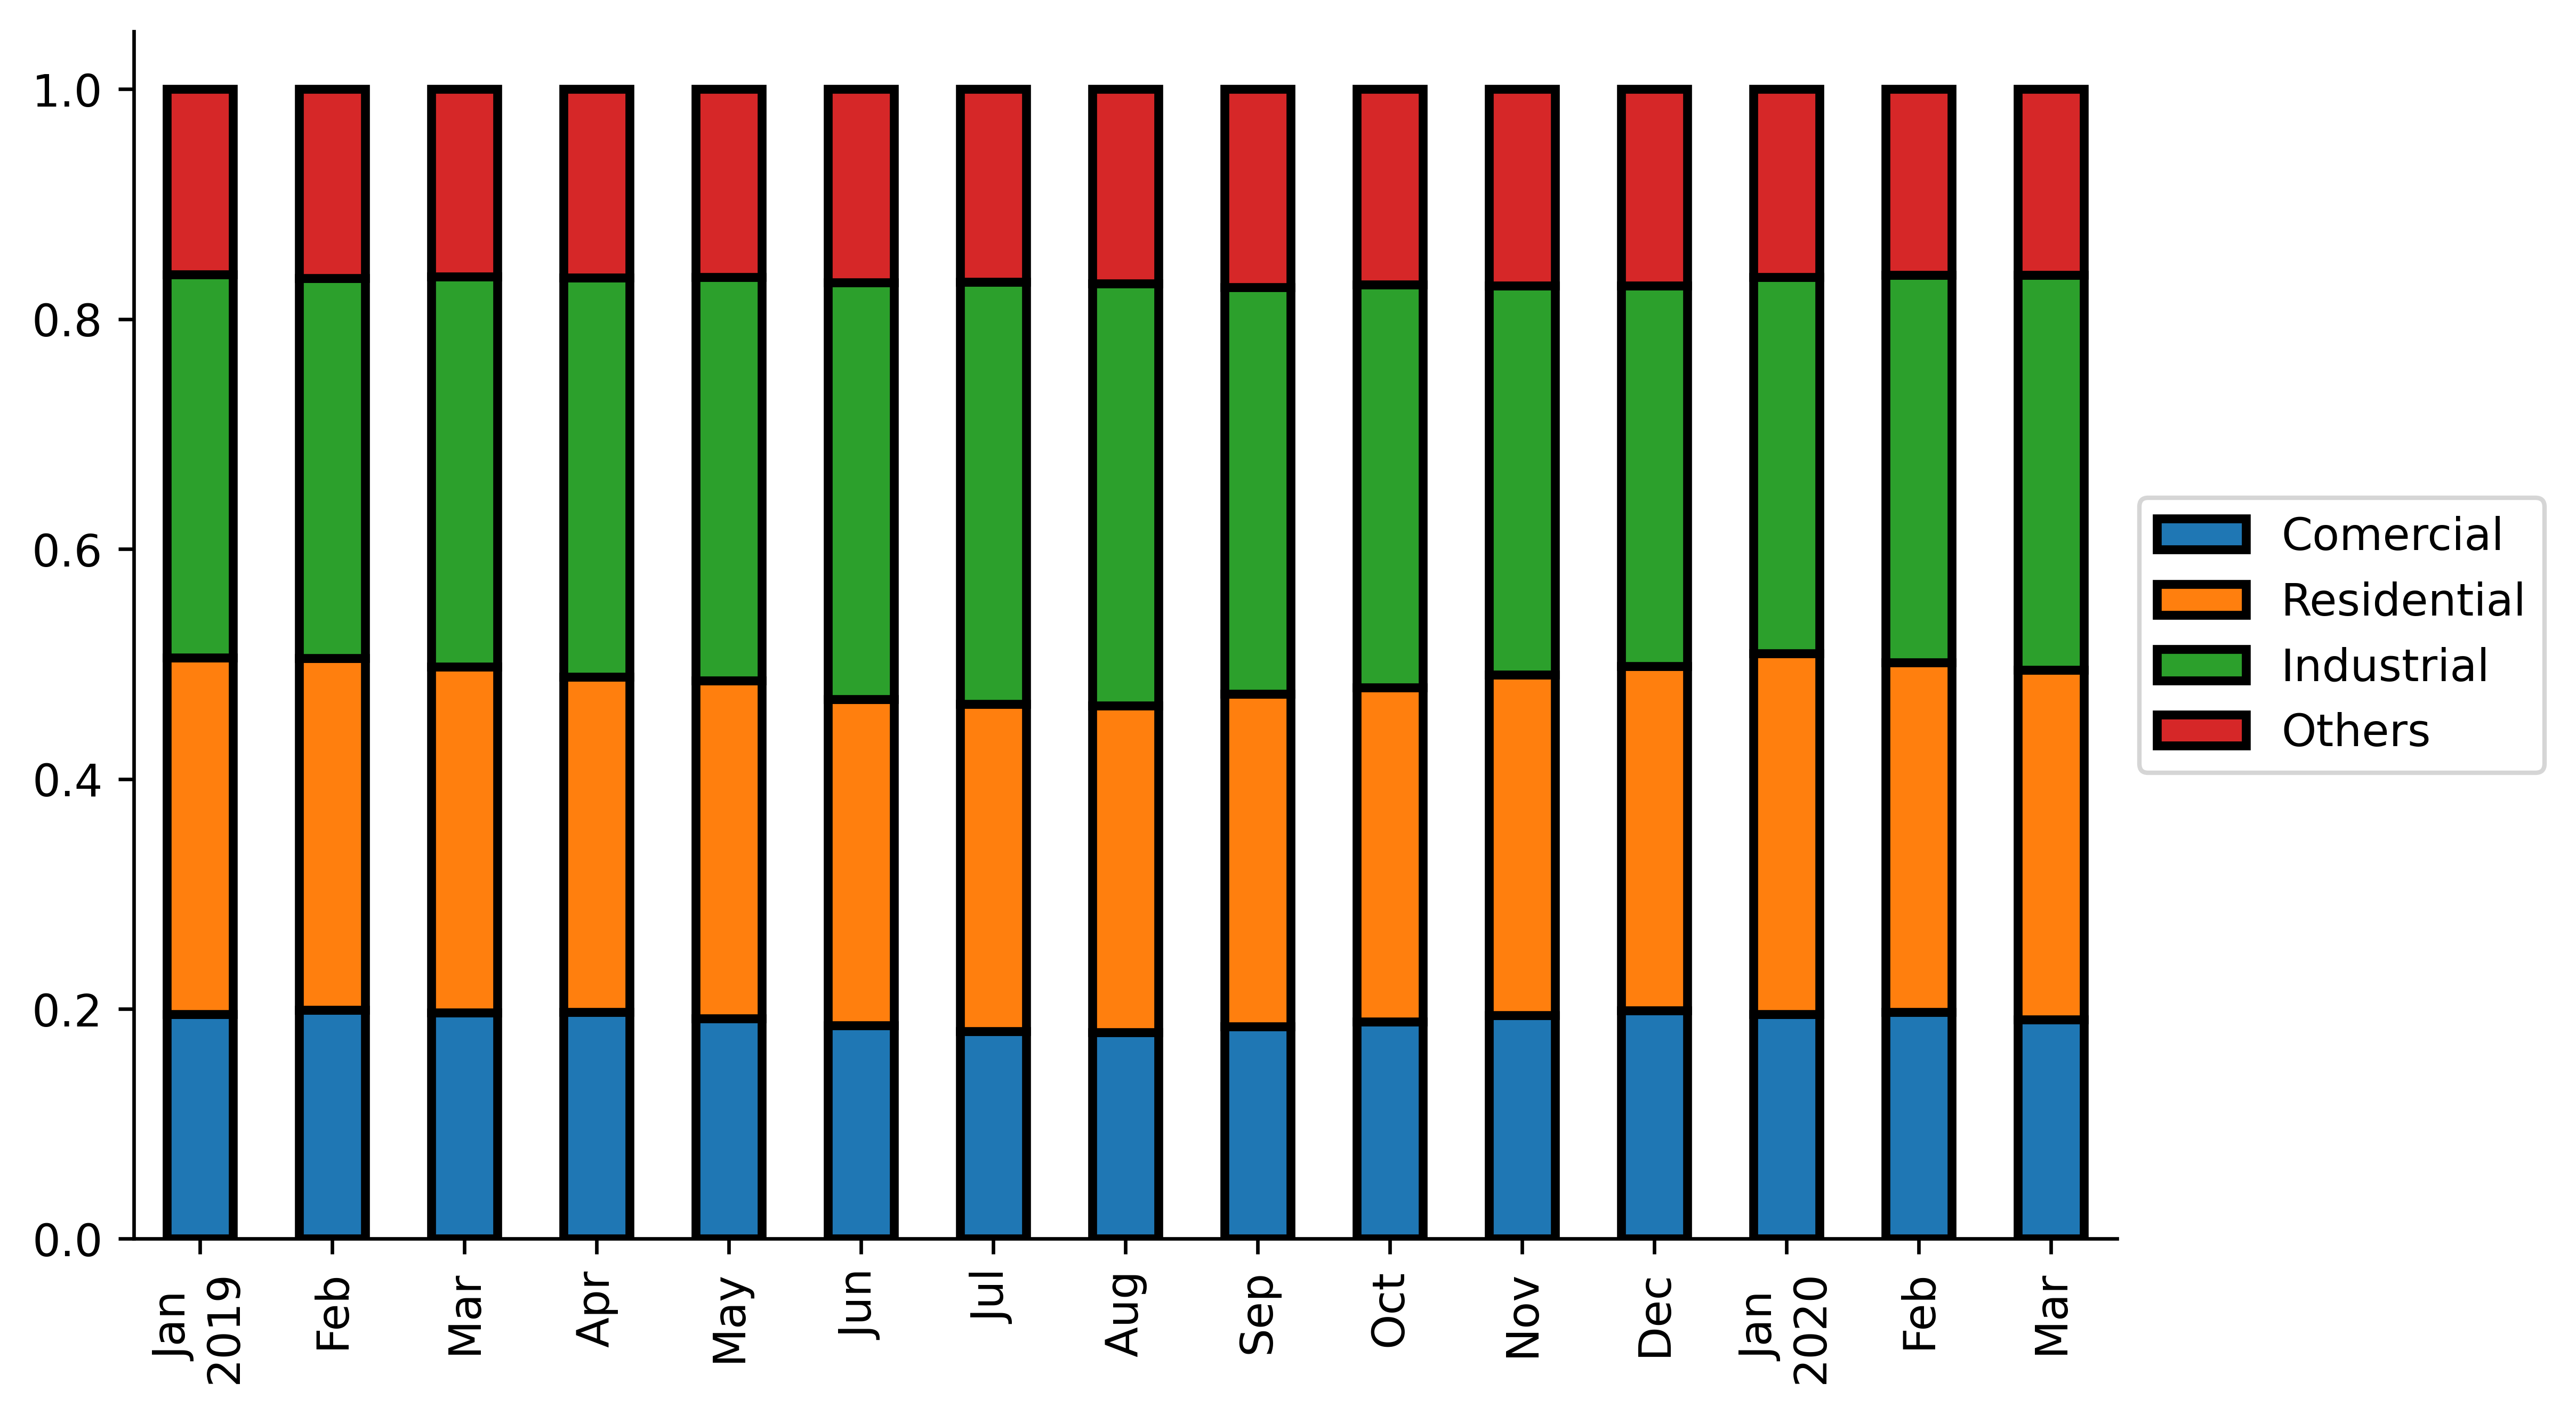
\includegraphics[width=.9\linewidth]{obipy-resources/62e383af79e91b63c7fc98dd7fb55b3c3ececcb9/b9bb93431770d5b32665b50dc4549f5f948c88a6.png}
\end{center}

\item Consumo Diário
\label{sec:org21c83f2}

\begin{verbatim}
<Figure size 2400x1500 with 2 Axes>
\end{verbatim}


\begin{center}
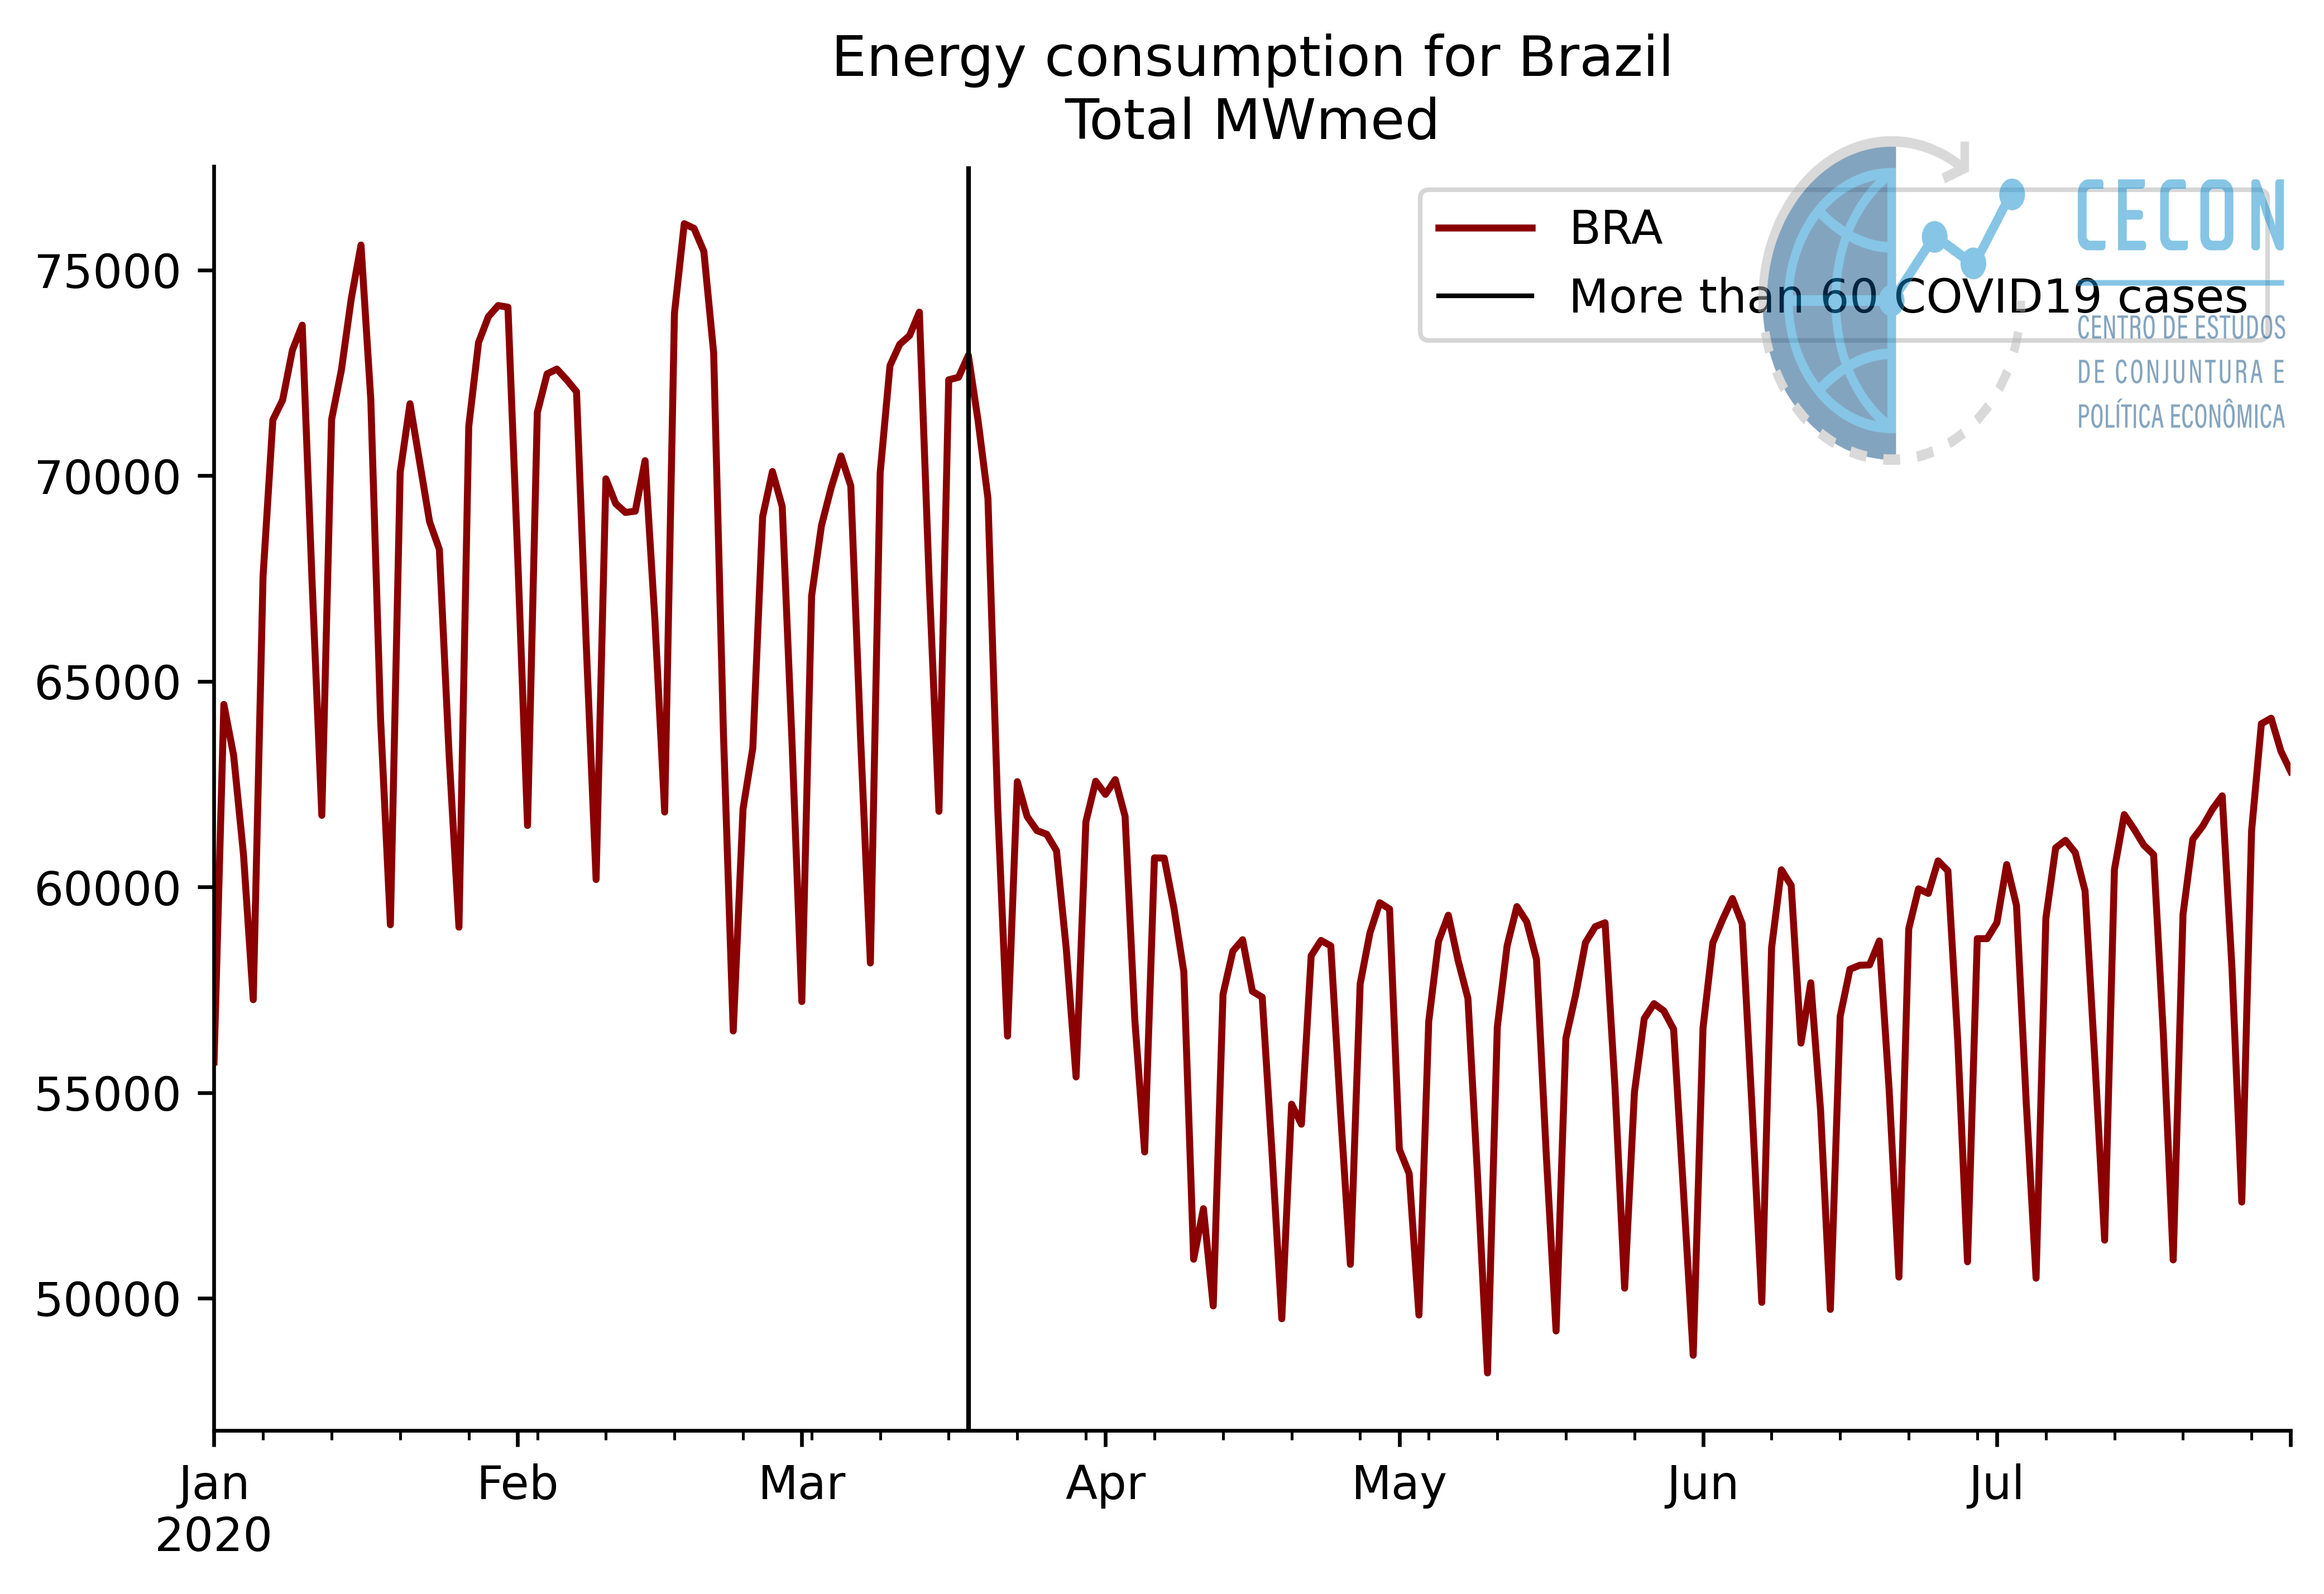
\includegraphics[width=.9\linewidth]{obipy-resources/62e383af79e91b63c7fc98dd7fb55b3c3ececcb9/77baa432ba2f44632060c841842355fcb8b83c23.png}
\end{center}

\begin{verbatim}
<Figure size 2400x1500 with 2 Axes>
\end{verbatim}


\begin{center}
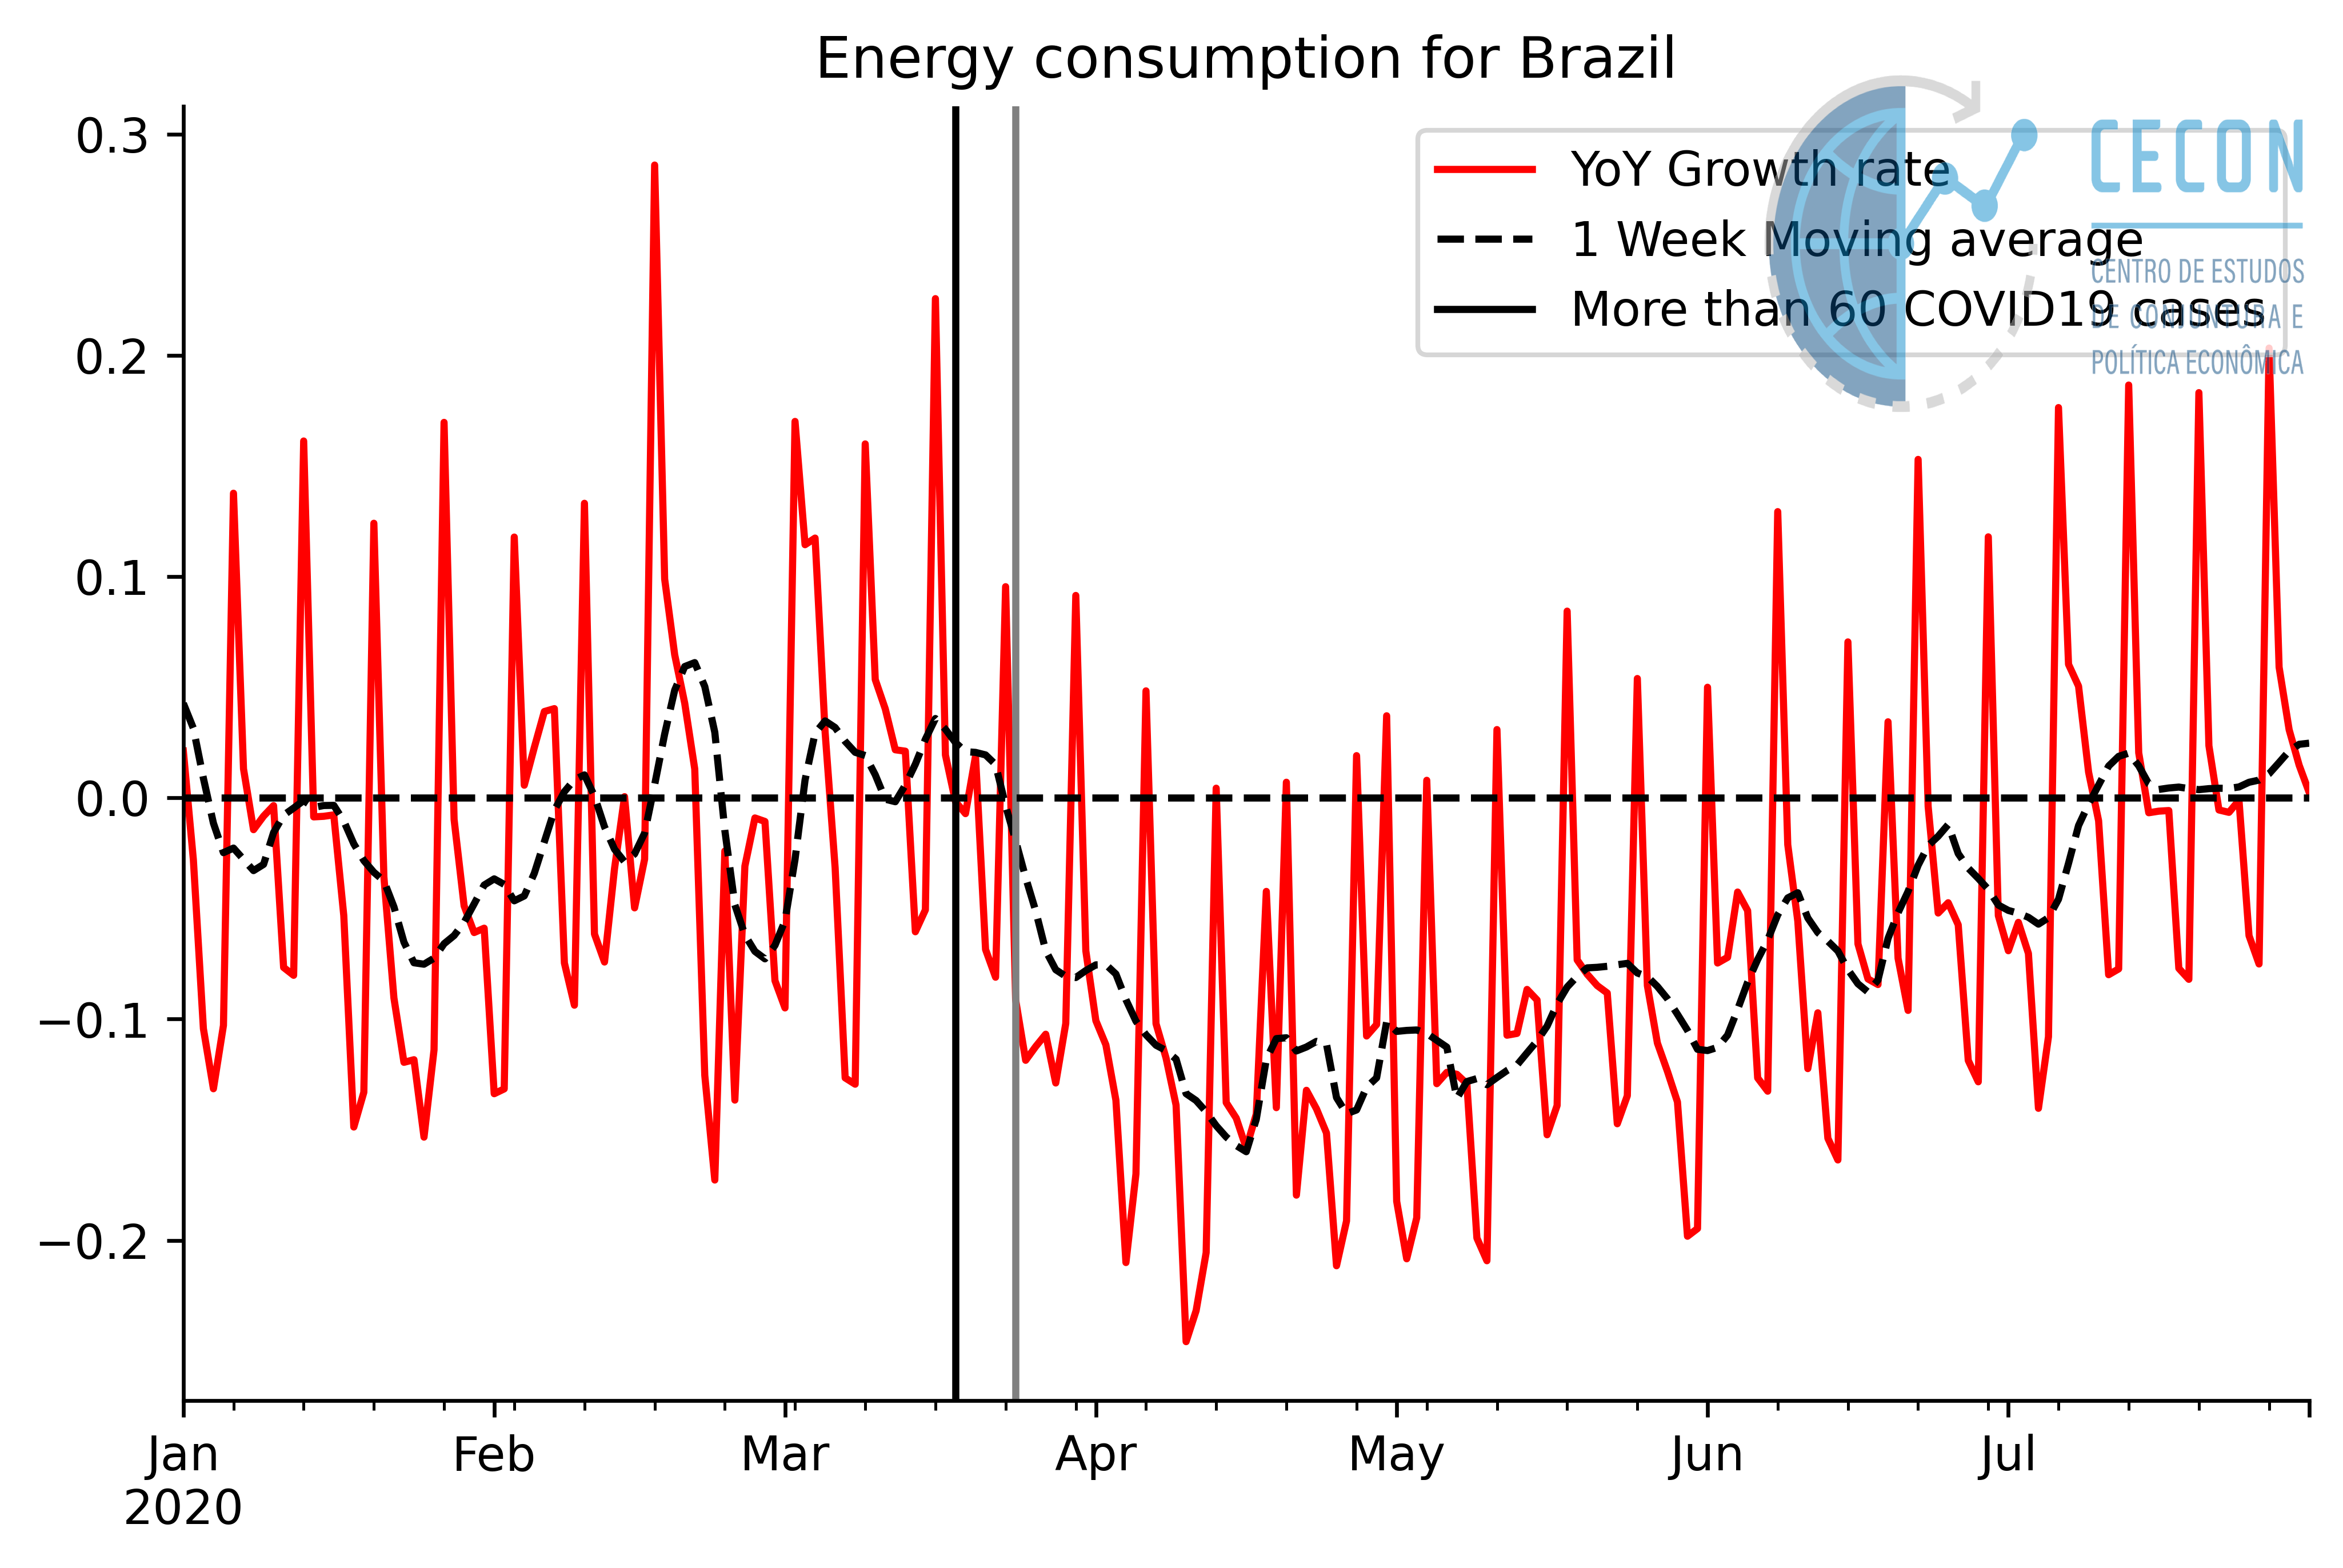
\includegraphics[width=.9\linewidth]{obipy-resources/62e383af79e91b63c7fc98dd7fb55b3c3ececcb9/d4289bac917b4c3c16dd2a44f65ca09392f8c087.png}
\end{center}

\begin{verbatim}
<Figure size 2400x1500 with 2 Axes>
\end{verbatim}


\begin{center}
\includegraphics[width=.9\linewidth]{obipy-resources/62e383af79e91b63c7fc98dd7fb55b3c3ececcb9/d84bd36ccade499cc39cebdae08232df8264d963.png}
\end{center}

\begin{verbatim}
<Figure size 2400x1500 with 2 Axes>
\end{verbatim}


\begin{center}
\includegraphics[width=.9\linewidth]{obipy-resources/62e383af79e91b63c7fc98dd7fb55b3c3ececcb9/09bb5c9f73ce423d9321f4fb6e122a99d548a06a.png}
\end{center}

\begin{verbatim}
<Figure size 2400x1500 with 2 Axes>
\end{verbatim}


\begin{center}
\includegraphics[width=.9\linewidth]{obipy-resources/62e383af79e91b63c7fc98dd7fb55b3c3ececcb9/f4a4030785824b36576994e7bc1b4ffd9e86a18c.png}
\end{center}

\begin{verbatim}
<Figure size 2400x1500 with 2 Axes>
\end{verbatim}


\begin{center}
\includegraphics[width=.9\linewidth]{obipy-resources/62e383af79e91b63c7fc98dd7fb55b3c3ececcb9/e7009b8bad859ec29423e1077cfdc4cfe98ad01d.png}
\end{center}
\end{enumerate}




\subsubsection{France: FRA}
\label{sec:org1261391}

<ipython-input-1-06392b792fc4>:74: UserWarning: This figure includes Axes that are not compatible with tight\_layout, so results might be incorrect.
  plt.tight\_layout()

\begin{verbatim}
<Figure size 2400x1500 with 4 Axes>
\end{verbatim}


\begin{center}
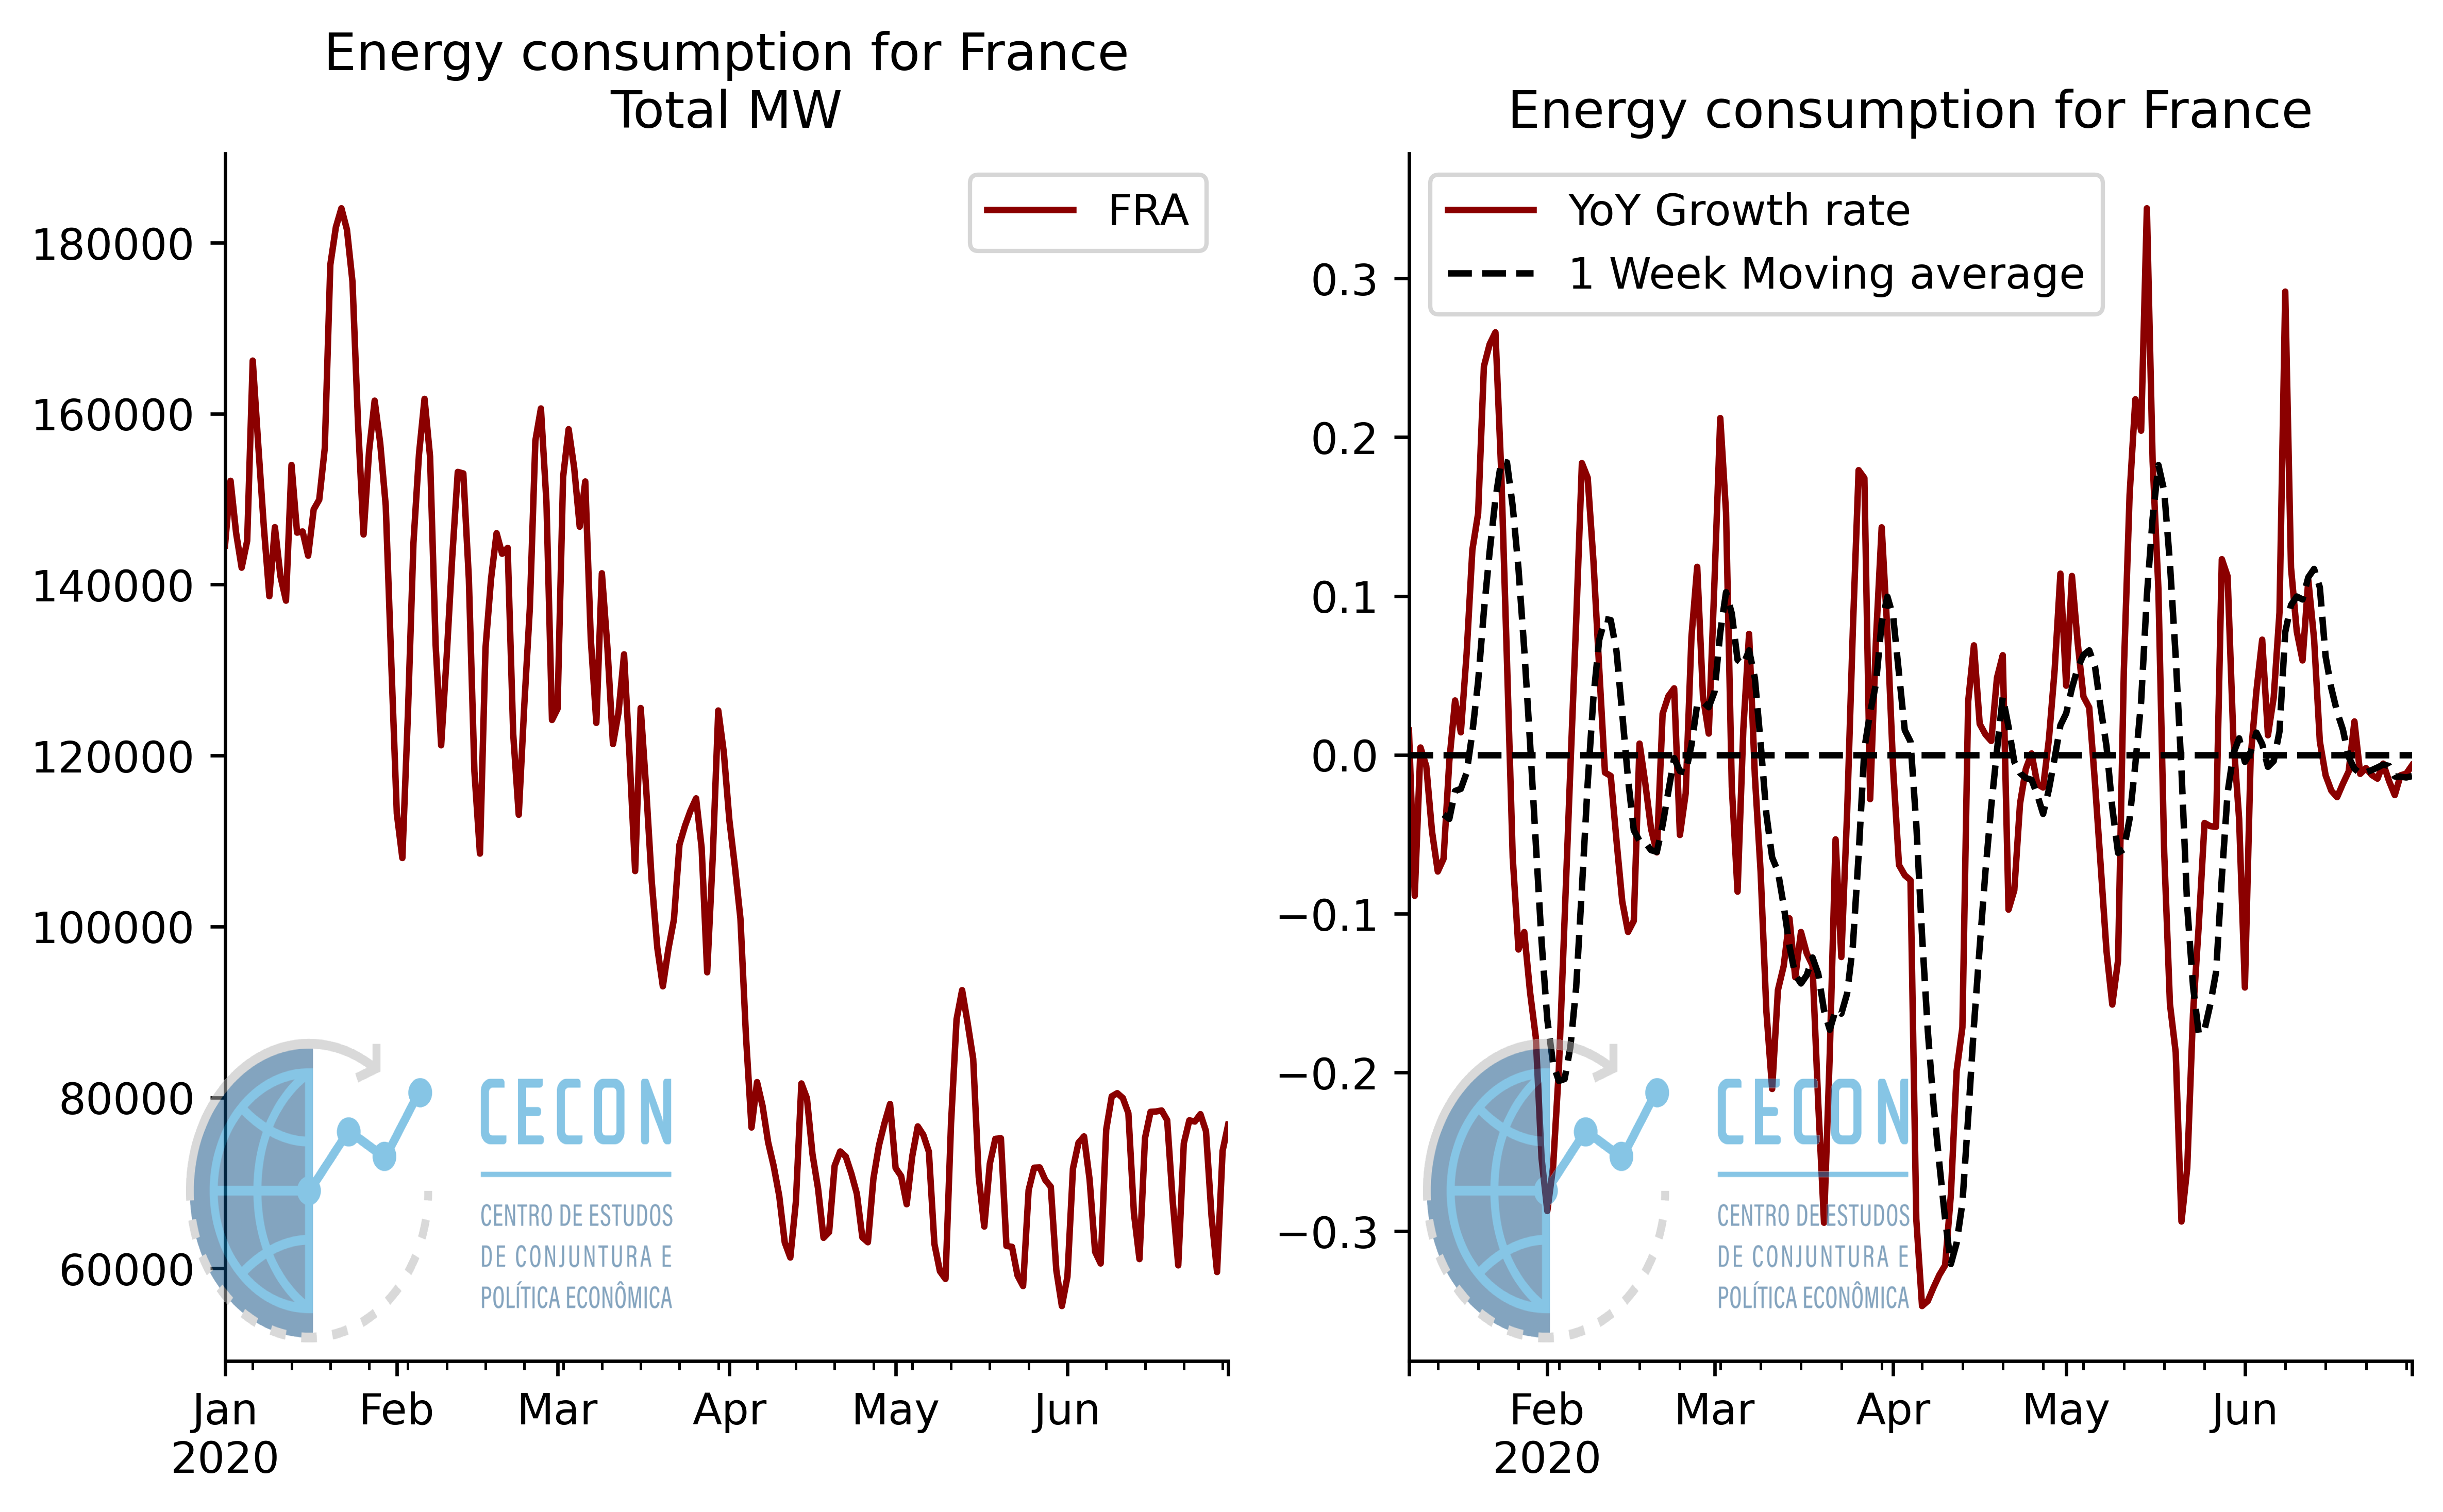
\includegraphics[width=.9\linewidth]{obipy-resources/62e383af79e91b63c7fc98dd7fb55b3c3ececcb9/325746abff053090d5f6fe9490ccdb4ba397472d.png}
\end{center}

\subsubsection{Spain: Spain}
\label{sec:org7a03652}

\textbf{Corrigir}

<ipython-input-1-06392b792fc4>:74: UserWarning: This figure includes Axes that are not compatible with tight\_layout, so results might be incorrect.
  plt.tight\_layout()

\begin{verbatim}
<Figure size 2400x1500 with 4 Axes>
\end{verbatim}


\begin{center}
\includegraphics[width=.9\linewidth]{obipy-resources/62e383af79e91b63c7fc98dd7fb55b3c3ececcb9/129d31512aa23532fa5d893d1f62677cb467d6e2.png}
\end{center}

\subsubsection{Austria: AUS}
\label{sec:orgec8e7e1}

<ipython-input-1-06392b792fc4>:74: UserWarning: This figure includes Axes that are not compatible with tight\_layout, so results might be incorrect.
  plt.tight\_layout()

\begin{verbatim}
(<Figure size 2400x1500 with 4 Axes>,
 array([<matplotlib.axes._subplots.AxesSubplot object at 0x7f29e07126a0>,
        <matplotlib.axes._subplots.AxesSubplot object at 0x7f29dd53ca30>],
       dtype=object))
\end{verbatim}


\begin{verbatim}
<Figure size 2400x1500 with 4 Axes>
\end{verbatim}


\begin{center}
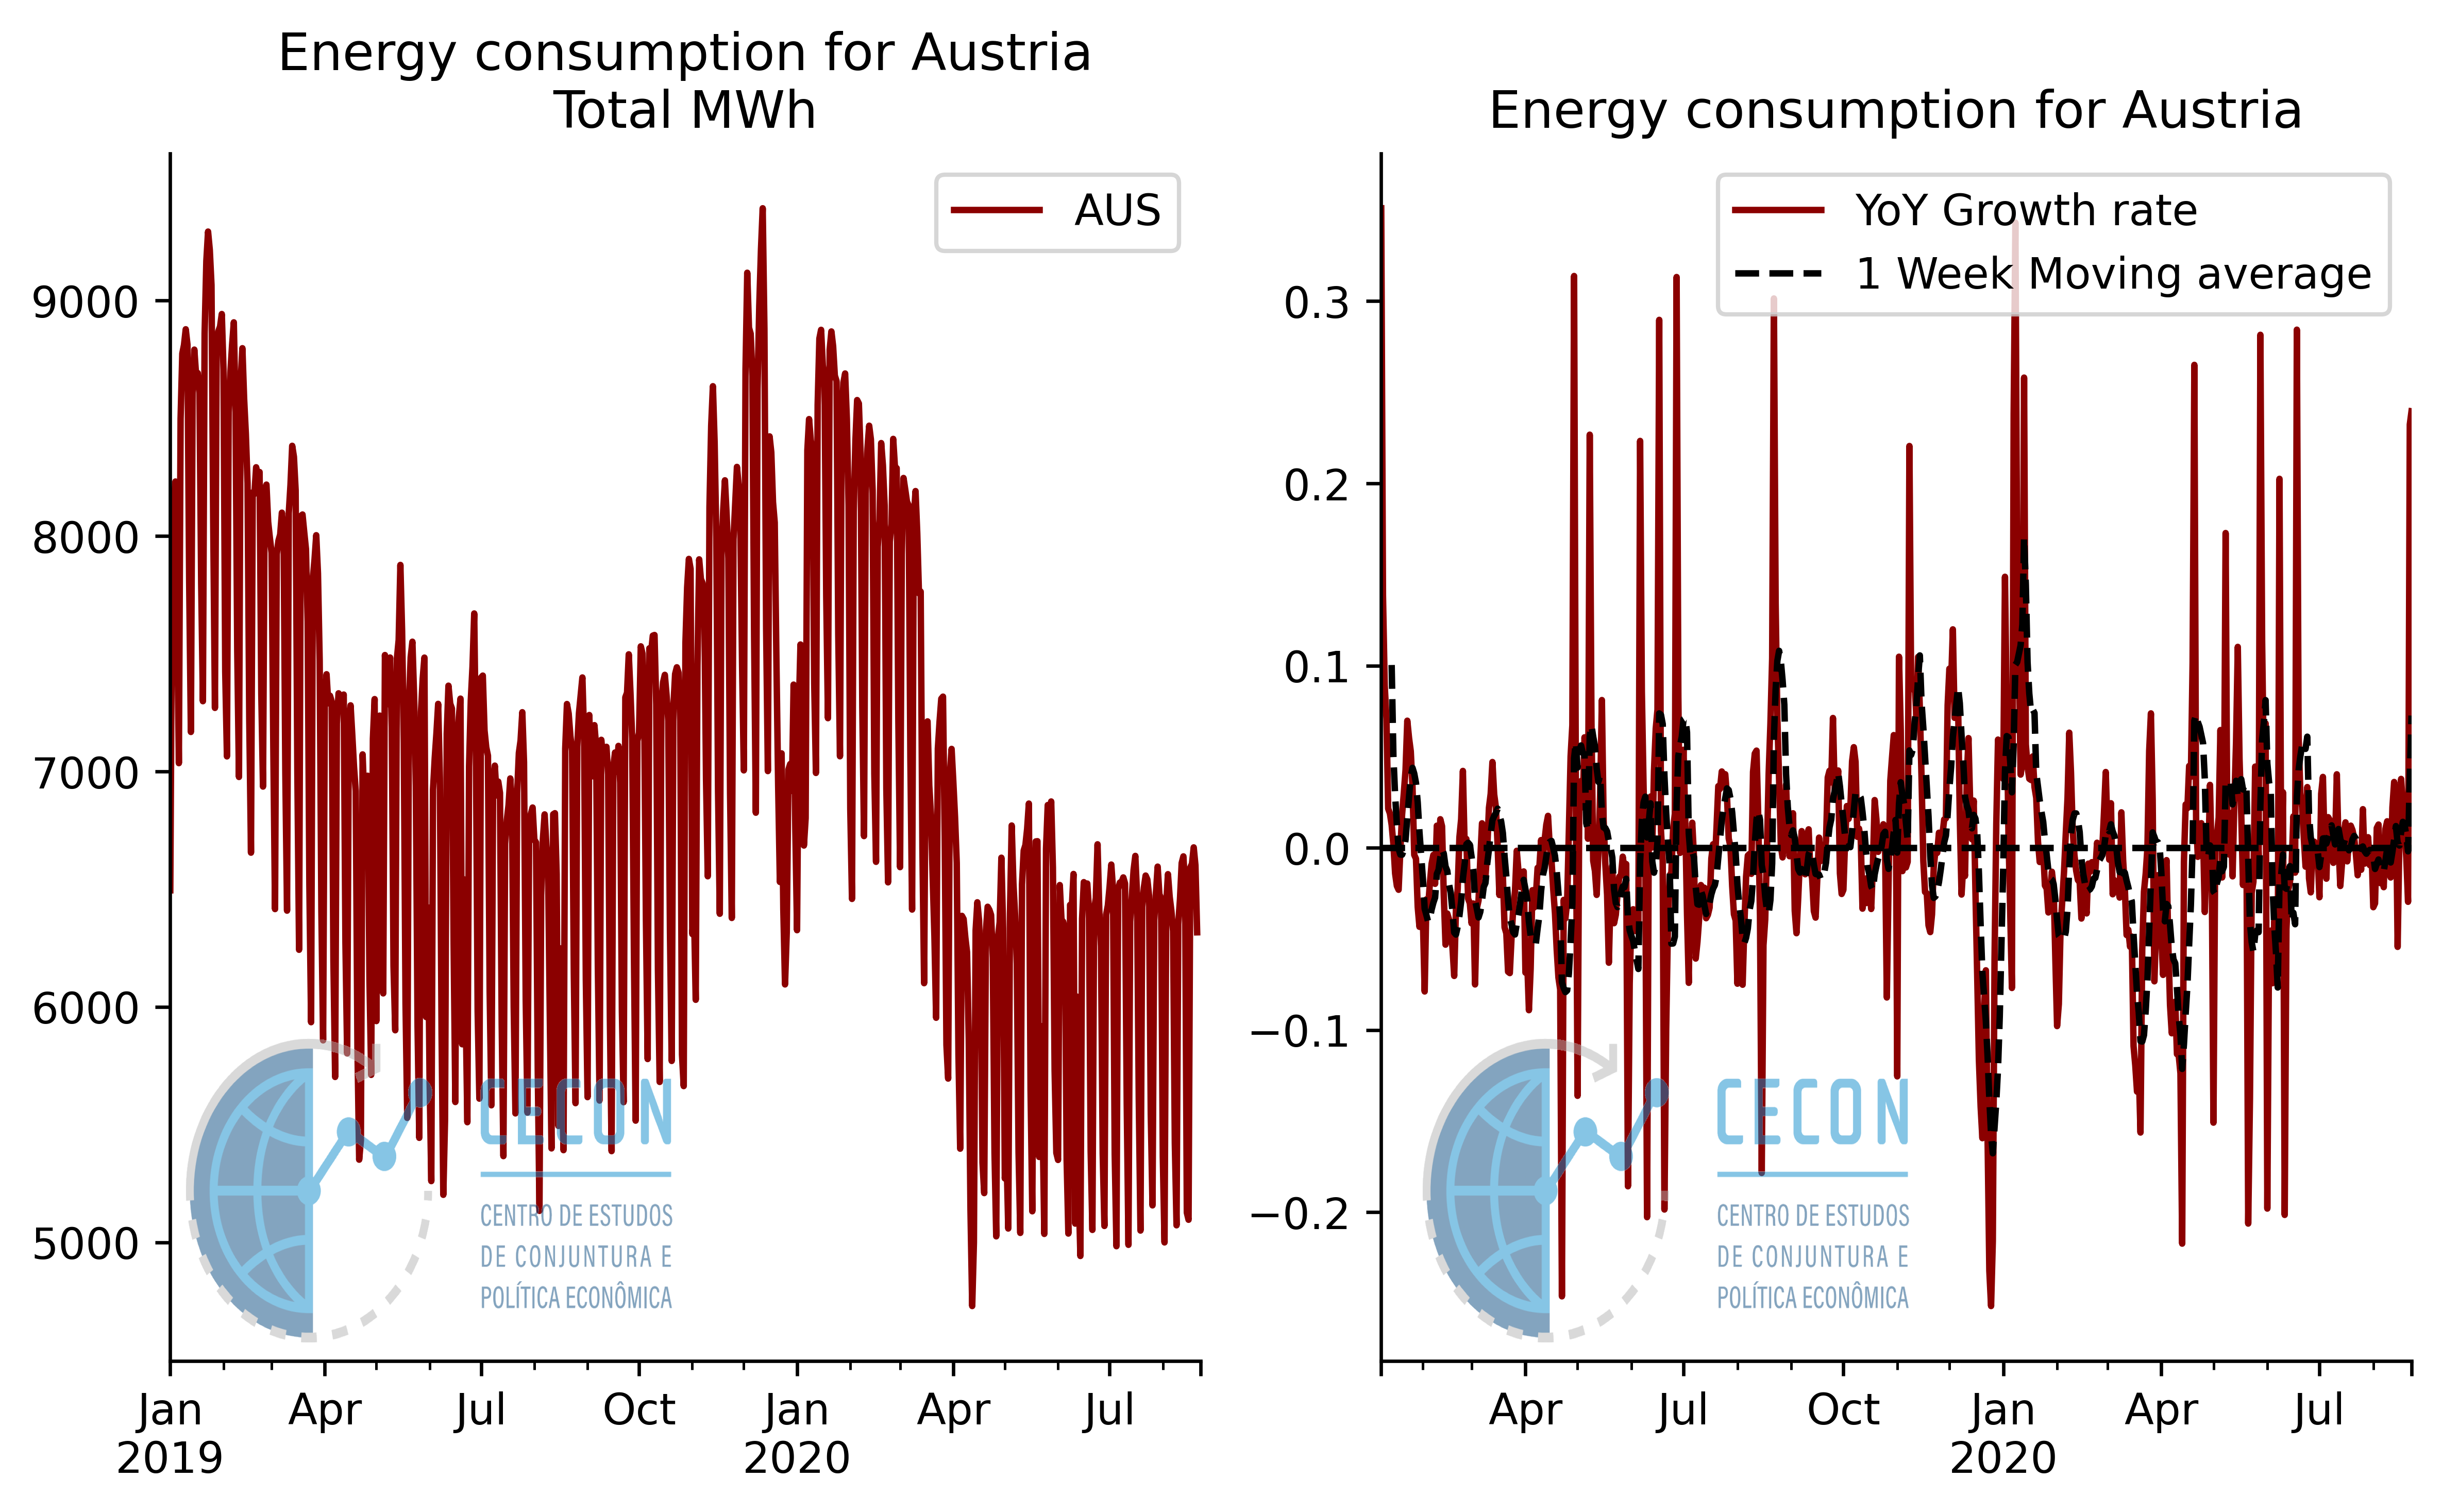
\includegraphics[width=.9\linewidth]{obipy-resources/62e383af79e91b63c7fc98dd7fb55b3c3ececcb9/9ef112a5872cc34e81a6bb8ef5d1a8c7b5fddf8e.png}
\end{center}

\subsubsection{Germany: GER}
\label{sec:org34d5574}

<ipython-input-1-06392b792fc4>:74: UserWarning: This figure includes Axes that are not compatible with tight\_layout, so results might be incorrect.
  plt.tight\_layout()

\begin{verbatim}
<Figure size 2400x1500 with 4 Axes>
\end{verbatim}


\begin{center}
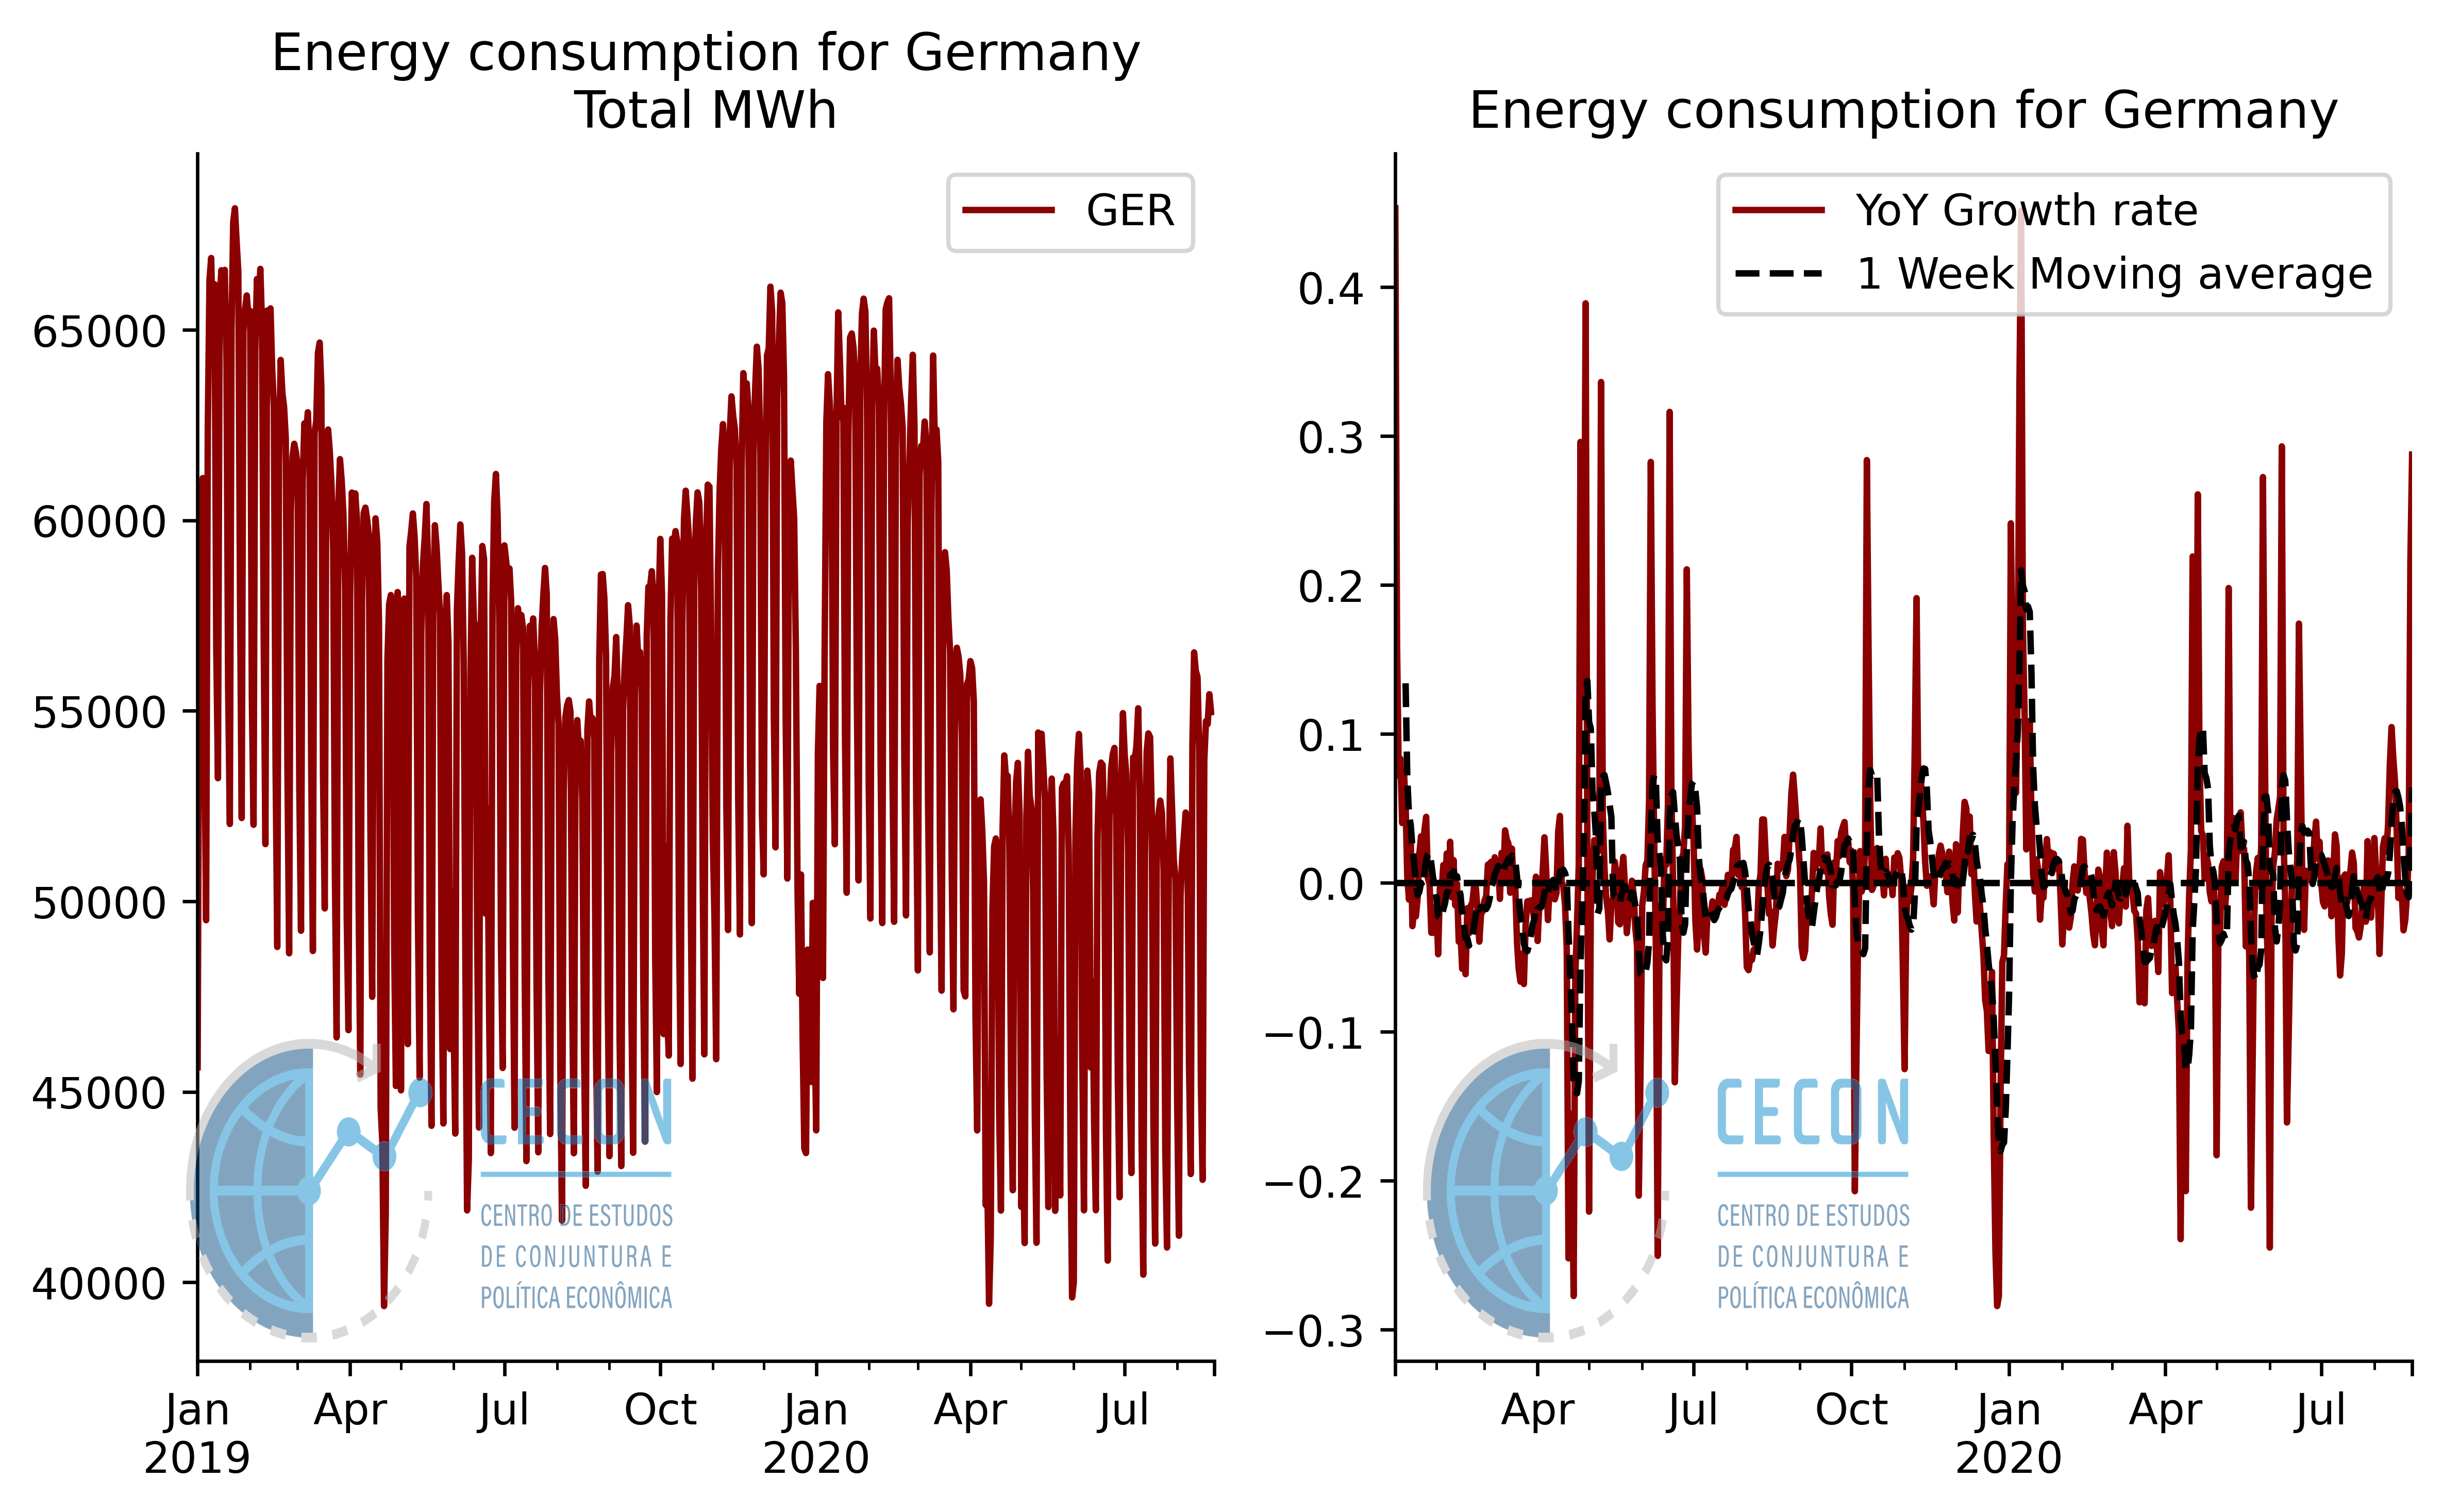
\includegraphics[width=.9\linewidth]{obipy-resources/62e383af79e91b63c7fc98dd7fb55b3c3ececcb9/94b114813ade8f5d4312e2e75f5b997a956c4a44.png}
\end{center}

\subsubsection{Luxemburg: LUX}
\label{sec:org1d0a876}

<ipython-input-1-06392b792fc4>:74: UserWarning: This figure includes Axes that are not compatible with tight\_layout, so results might be incorrect.
  plt.tight\_layout()

\begin{verbatim}
<Figure size 2400x1500 with 4 Axes>
\end{verbatim}


\begin{center}
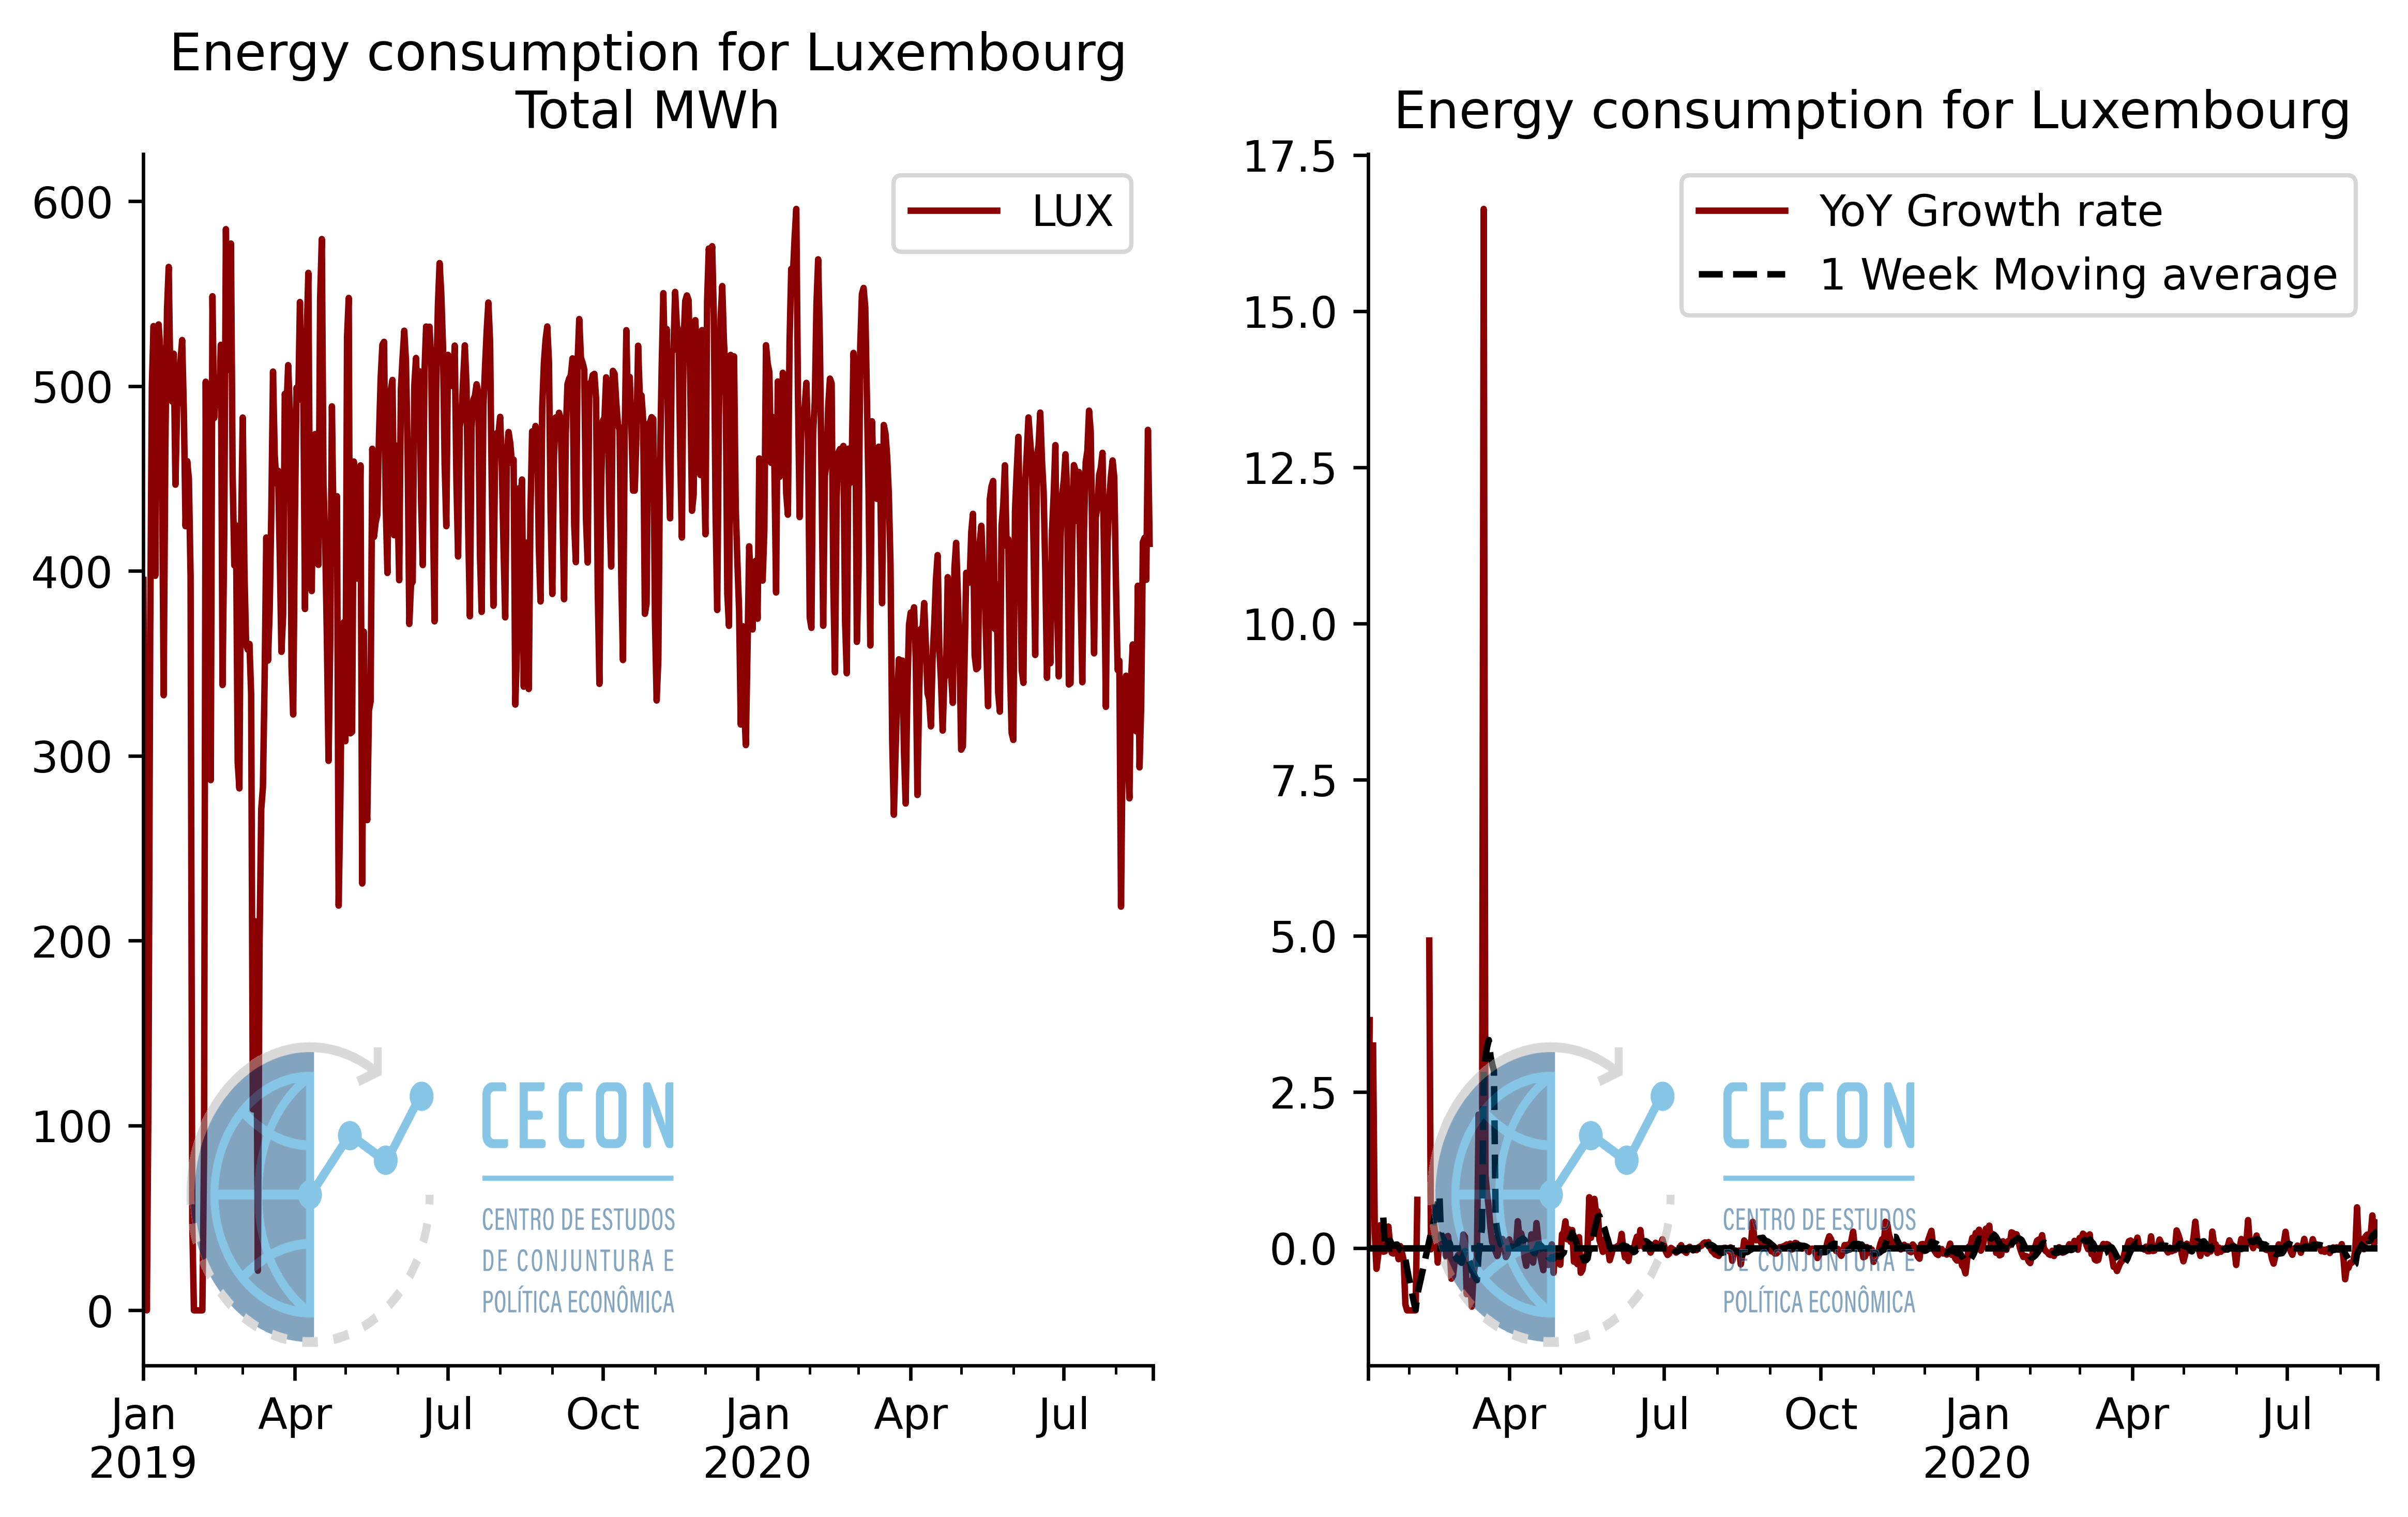
\includegraphics[width=.9\linewidth]{obipy-resources/62e383af79e91b63c7fc98dd7fb55b3c3ececcb9/9106e308f42f1f76c029539778f3952a7f562f15.png}
\end{center}


\subsection{Aruoba-Diebold-Scotti Business Conditions Index}
\label{sec:org77ea1f3}

\begin{verbatim}
<Figure size 2400x1500 with 2 Axes>
\end{verbatim}


\begin{center}
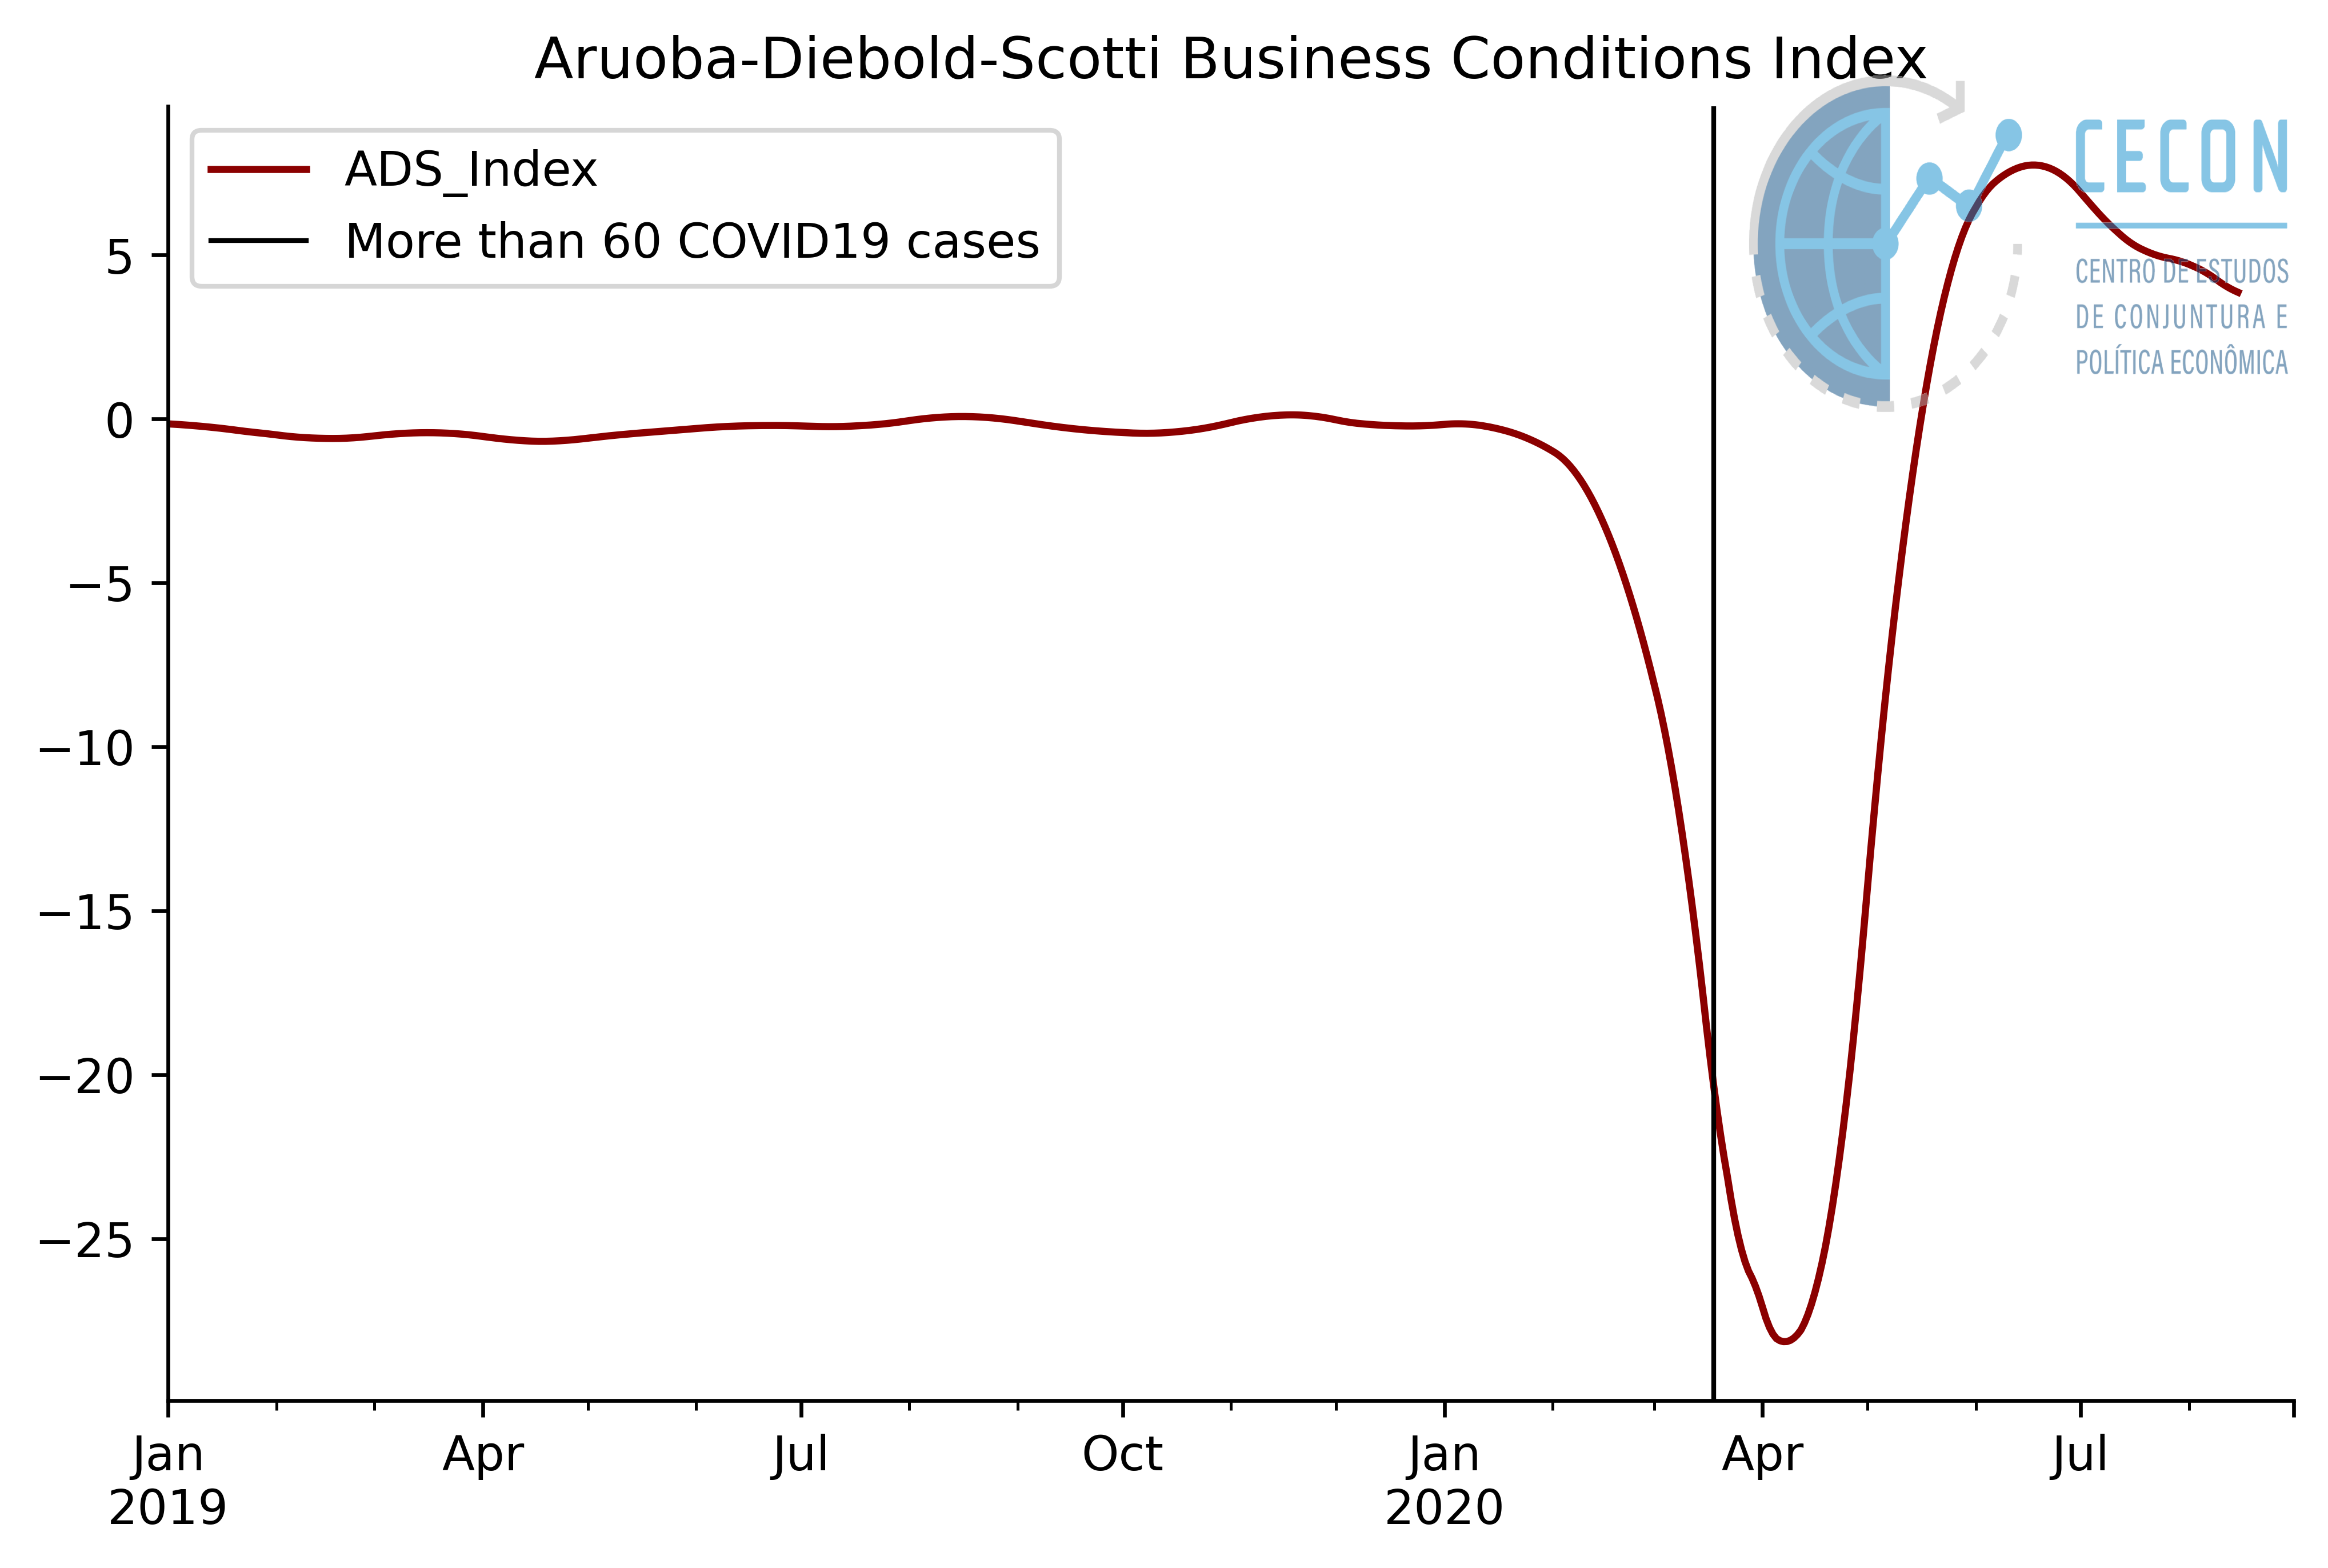
\includegraphics[width=.9\linewidth]{obipy-resources/62e383af79e91b63c7fc98dd7fb55b3c3ececcb9/cf14fa691a64e7d5e47f44565dc9f5363854ad6e.png}
\end{center}

\section{Confiança, Indicadores de antecedentes e de Risco}
\label{sec:org77ba10f}

\subsection{Confiança}
\label{sec:org333aecb}

\emph{home/gpetrini}.local/lib/python3.8/site-packages/pandas\_datareader/compat/\_\_init\_\_.py:7: FutureWarning: pandas.util.testing is deprecated. Use the functions in the public API at pandas.testing instead.
  from pandas.util.testing import assert\_frame\_equal

\subsubsection{Sondagem Conjuntural Mensal}
\label{sec:org5e2f7c6}

\begin{verbatim}
<Figure size 576x360 with 2 Axes>
\end{verbatim}


\begin{center}
\includegraphics[width=.9\linewidth]{obipy-resources/62e383af79e91b63c7fc98dd7fb55b3c3ececcb9/8a25efae9231056627de37bc9a8ba5ccbde9d524.png}
\end{center}

\subsubsection{Sondagens de serviços}
\label{sec:org779f45b}

\begin{verbatim}
<Figure size 576x360 with 2 Axes>
\end{verbatim}


\begin{center}
\includegraphics[width=.9\linewidth]{obipy-resources/62e383af79e91b63c7fc98dd7fb55b3c3ececcb9/b8884fa0650b2c2def8988d527bbeadc933c5cac.png}
\end{center}


\subsubsection{Sondagem do comércio}
\label{sec:org258e7b7}

\begin{verbatim}
<Figure size 576x360 with 2 Axes>
\end{verbatim}


\begin{center}
\includegraphics[width=.9\linewidth]{obipy-resources/62e383af79e91b63c7fc98dd7fb55b3c3ececcb9/3ff0b698bb29513242319b177af1c0a29f2409fb.png}
\end{center}

\subsubsection{Sondagem da construção}
\label{sec:orgf74bcb7}

\begin{verbatim}
<Figure size 576x360 with 2 Axes>
\end{verbatim}


\begin{center}
\includegraphics[width=.9\linewidth]{obipy-resources/62e383af79e91b63c7fc98dd7fb55b3c3ececcb9/3457739c82986a176433fecd8d1a1f246d2a7529.png}
\end{center}

\subsubsection{Sondagem industrial CNI}
\label{sec:org8386586}


\begin{enumerate}
\item Volume de produção
\label{sec:org5ef87af}

\begin{verbatim}
<Figure size 576x360 with 2 Axes>
\end{verbatim}


\begin{center}
\includegraphics[width=.9\linewidth]{obipy-resources/62e383af79e91b63c7fc98dd7fb55b3c3ececcb9/190c8feb1adde26683c40b65c19eda8712bdf352.png}
\end{center}

\item Evolução do Emprego
\label{sec:orgaa3b896}

\begin{verbatim}
<Figure size 576x360 with 2 Axes>
\end{verbatim}


\begin{center}
\includegraphics[width=.9\linewidth]{obipy-resources/62e383af79e91b63c7fc98dd7fb55b3c3ececcb9/433a12bb8c07cd8a313c63f9fd67450df4f145d1.png}
\end{center}


\item NUCI
\label{sec:org2c65816}

\noindent\rule{\textwidth}{0.5pt}
NameError                                 Traceback (most recent call last)
<ipython-input-9-f5ad43e4d316> in <module>
      9     lw = 2.5
     10 )
---> 11 ax.axvline(x = corona, color='black', ls='--', lw=1, label='Início do isolamento em SP\n(24 de março)')
     12 ax.legend(loc='center left', bbox\_to\_anchor=(1, 0.5))
     13 ax2 = plt.axes([0.135,0.135,0.2,0.2])

NameError: name 'corona' is not defined

\begin{verbatim}
<Figure size 576x360 with 1 Axes>
\end{verbatim}


\begin{center}
\includegraphics[width=.9\linewidth]{obipy-resources/62e383af79e91b63c7fc98dd7fb55b3c3ececcb9/4f9cc42543a2d57e44823ebbc3883c2e481fd6ce.png}
\end{center}

\item NUCI Efeito-Usual
\label{sec:org9c836b0}

\begin{verbatim}
<Figure size 576x360 with 2 Axes>
\end{verbatim}


\begin{center}
\includegraphics[width=.9\linewidth]{obipy-resources/62e383af79e91b63c7fc98dd7fb55b3c3ececcb9/ab35061abeddc7db0e957552c2e5902ec47c321e.png}
\end{center}

\item Evolução de estoques
\label{sec:orgdabc316}

\noindent\rule{\textwidth}{0.5pt}
NameError                                 Traceback (most recent call last)
<ipython-input-11-bd6352613dfc> in <module>
      9     lw = 2.5
     10 )
---> 11 ax.axvline(x = corona, color='black', ls='--', lw=1, label='Início do isolamento em SP\n(24 de março)')
     12 ax.legend(loc='center left', bbox\_to\_anchor=(1, 0.5))
     13 ax2 = plt.axes([0.135,0.135,0.2,0.2])

NameError: name 'corona' is not defined

\begin{verbatim}
<Figure size 576x360 with 1 Axes>
\end{verbatim}


\begin{center}
\includegraphics[width=.9\linewidth]{obipy-resources/62e383af79e91b63c7fc98dd7fb55b3c3ececcb9/ee2e0ef4d86c219085ca9aa8eb1df02445fc4000.png}
\end{center}

\item Estoques efetivos
\label{sec:org0ba75a3}

\begin{verbatim}
<Figure size 576x360 with 2 Axes>
\end{verbatim}


\begin{center}
\includegraphics[width=.9\linewidth]{obipy-resources/62e383af79e91b63c7fc98dd7fb55b3c3ececcb9/5af9aa5b5d2d37338f8964e8451506dc7e1e4c53.png}
\end{center}

\item Expectativa de Demanda
\label{sec:orgc8f0683}

\begin{verbatim}
<Figure size 576x360 with 2 Axes>
\end{verbatim}


\begin{center}
\includegraphics[width=.9\linewidth]{obipy-resources/62e383af79e91b63c7fc98dd7fb55b3c3ececcb9/26cc0738ba131ee757deed5c9a90853d5ee9f94e.png}
\end{center}

\item Expectativa de Exportação
\label{sec:org16ae293}

\begin{verbatim}
<Figure size 576x360 with 2 Axes>
\end{verbatim}


\begin{center}
\includegraphics[width=.9\linewidth]{obipy-resources/62e383af79e91b63c7fc98dd7fb55b3c3ececcb9/fb4b9ac7d589651ae78f9cb61d45452a1c20cffc.png}
\end{center}

\item Expectativa de compra de matéria-prima
\label{sec:org9aebe25}


\begin{verbatim}
<Figure size 576x360 with 2 Axes>
\end{verbatim}


\begin{center}
\includegraphics[width=.9\linewidth]{obipy-resources/62e383af79e91b63c7fc98dd7fb55b3c3ececcb9/1613740d59e200de1ed90cd00658aa98d76fccf5.png}
\end{center}

\item Expectativa de emprego
\label{sec:org8c265f6}

\begin{verbatim}
<Figure size 576x360 with 2 Axes>
\end{verbatim}


\begin{center}
\includegraphics[width=.9\linewidth]{obipy-resources/62e383af79e91b63c7fc98dd7fb55b3c3ececcb9/0a3e42b80d0eaee635069c6ee57ed7964c2109a5.png}
\end{center}

\item Expectativa de investimento
\label{sec:org75cdb42}

\begin{verbatim}
<Figure size 576x360 with 2 Axes>
\end{verbatim}


\begin{center}
\includegraphics[width=.9\linewidth]{obipy-resources/62e383af79e91b63c7fc98dd7fb55b3c3ececcb9/30862091e2f2a14c212ea33ba93271329494e654.png}
\end{center}

\item Lucro Operacional
\label{sec:orga3a2b9c}


\begin{verbatim}
<Figure size 576x360 with 2 Axes>
\end{verbatim}


\begin{center}
\includegraphics[width=.9\linewidth]{obipy-resources/62e383af79e91b63c7fc98dd7fb55b3c3ececcb9/e275139cf83d1eda006dc4b30dbadda64774133a.png}
\end{center}

\item Situação Financeira
\label{sec:org19838eb}

\begin{verbatim}
<Figure size 576x360 with 2 Axes>
\end{verbatim}


\begin{center}
\includegraphics[width=.9\linewidth]{obipy-resources/62e383af79e91b63c7fc98dd7fb55b3c3ececcb9/22bcc5c077b1cb4dcefe2a59c9d0116b7de82c73.png}
\end{center}


\item Acesso a Crédito
\label{sec:org2f30ff7}

\begin{verbatim}
<Figure size 576x360 with 2 Axes>
\end{verbatim}


\begin{center}
\includegraphics[width=.9\linewidth]{obipy-resources/62e383af79e91b63c7fc98dd7fb55b3c3ececcb9/2ded59c6ca4da81dd78c570c38c84f405c7e65b6.png}
\end{center}
\end{enumerate}

\subsection{Indicadores de antecedente}
\label{sec:orgd2959e3}

\subsubsection{Composite Leading index (\href{https://stats.oecd.org/Index.aspx?DataSetCode=MEI\_CLI}{CLI})}
\label{sec:org73e7a77}

WARNING:root:OECD + Major Six NME not found in regex
WARNING:root:Major Five Asia not found in regex
WARNING:root:Four Big European not found in regex
WARNING:root:G7 not found in ISO2
WARNING:root:NAFTA not found in regex
WARNING:root:OECD - Total not found in regex
WARNING:root:OECD - Europe not found in regex
WARNING:root:Euro area (19 countries) not found in regex
WARNING:root:OECD total  not found in regex

\begin{verbatim}
<Figure size 576x360 with 1 Axes>
\end{verbatim}


\begin{center}
\includegraphics[width=.9\linewidth]{obipy-resources/62e383af79e91b63c7fc98dd7fb55b3c3ececcb9/4cfcc53fcf196fc11008c55606296df35b25db0f.png}
\end{center}


\subsubsection{Consumer Confidence index (\href{https://stats.oecd.org/Index.aspx?DataSetCode=MEI\_CCI}{CCI})}
\label{sec:org7bfb986}

\emph{home/gpetrini}.local/lib/python3.8/site-packages/pandas/core/indexing.py:1762: PerformanceWarning: indexing past lexsort depth may impact performance.
  return self.\_getitem\_tuple(key)
WARNING:root:OECD + Major Six NME not found in regex
WARNING:root:Major Five Asia not found in regex
WARNING:root:Four Big European not found in regex
WARNING:root:G7 not found in ISO2
WARNING:root:NAFTA not found in regex
WARNING:root:OECD - Total not found in regex
WARNING:root:OECD - Europe not found in regex
WARNING:root:Euro area (19 countries) not found in regex
WARNING:root:OECD total  not found in regex

\begin{verbatim}
<Figure size 576x360 with 1 Axes>
\end{verbatim}


\begin{center}
\includegraphics[width=.9\linewidth]{obipy-resources/62e383af79e91b63c7fc98dd7fb55b3c3ececcb9/e5460aa82c2c15556a69dea566dab149d25f8cf9.png}
\end{center}

\subsection{Risco}
\label{sec:org3c5e8d2}

\subsubsection{EMBI+ (JP Morgan)}
\label{sec:orgae054b2}

\begin{verbatim}
<Figure size 576x360 with 2 Axes>
\end{verbatim}


\begin{center}
\includegraphics[width=.9\linewidth]{obipy-resources/62e383af79e91b63c7fc98dd7fb55b3c3ececcb9/8b49720c67f868a07188ddeb0242c5bb3791d599.png}
\end{center}


\subsection{Incerteza}
\label{sec:org4820402}

\emph{home/gpetrini}.local/lib/python3.8/site-packages/pandas\_datareader/compat/\_\_init\_\_.py:7: FutureWarning: pandas.util.testing is deprecated. Use the functions in the public API at pandas.testing instead.
  from pandas.util.testing import assert\_frame\_equal


\subsubsection{Indicador de Incerteza (IIE-Br)}
\label{sec:org90386f0}

\begin{verbatim}
<Figure size 2400x1500 with 2 Axes>
\end{verbatim}


\begin{center}
\includegraphics[width=.9\linewidth]{obipy-resources/62e383af79e91b63c7fc98dd7fb55b3c3ececcb9/98ebb468eb299bda8f1859499b3331c18b937130.png}
\end{center}


\subsubsection{Indicador de Confiança Empresarial}
\label{sec:orga29ed5c}

\begin{verbatim}
<Figure size 2400x1500 with 2 Axes>
\end{verbatim}


\begin{center}
\includegraphics[width=.9\linewidth]{obipy-resources/62e383af79e91b63c7fc98dd7fb55b3c3ececcb9/925a5b9efaef4a764499db16a51227974403bd49.png}
\end{center}

\section{Atividade}
\label{sec:orgefc823a}

\subsection{Crédito}
\label{sec:org42f9407}

\emph{home/gpetrini}.local/lib/python3.8/site-packages/pandas\_datareader/compat/\_\_init\_\_.py:7: FutureWarning: pandas.util.testing is deprecated. Use the functions in the public API at pandas.testing instead.
  from pandas.util.testing import assert\_frame\_equal

\subsubsection{Saldo}
\label{sec:orgd6b72ed}

\begin{enumerate}
\item Pessoa jurídica
\label{sec:orgca2c631}

\begin{verbatim}
<Figure size 576x360 with 2 Axes>
\end{verbatim}


\begin{center}
\includegraphics[width=.9\linewidth]{obipy-resources/62e383af79e91b63c7fc98dd7fb55b3c3ececcb9/feb0adea384d3519399baabeaaea53ffd62ea8b2.png}
\end{center}


\begin{verbatim}
<Figure size 576x360 with 2 Axes>
\end{verbatim}


\begin{center}
\includegraphics[width=.9\linewidth]{obipy-resources/62e383af79e91b63c7fc98dd7fb55b3c3ececcb9/814881da38842cb94f0fd6474ddd70e90bd352da.png}
\end{center}

\item Pessoa física
\label{sec:orgcf2c8fc}

\begin{verbatim}
<Figure size 576x360 with 2 Axes>
\end{verbatim}


\begin{center}
\includegraphics[width=.9\linewidth]{obipy-resources/62e383af79e91b63c7fc98dd7fb55b3c3ececcb9/631784503e9693a2f771311b1a337a6f61bd3bcb.png}
\end{center}

\begin{verbatim}
<Figure size 576x360 with 2 Axes>
\end{verbatim}


\begin{center}
\includegraphics[width=.9\linewidth]{obipy-resources/62e383af79e91b63c7fc98dd7fb55b3c3ececcb9/840ea262d5c525c19284dff3d45594fc372c02d1.png}
\end{center}

\item Crédito ampliado
\label{sec:orgea5075c}

\begin{verbatim}
<Figure size 576x360 with 2 Axes>
\end{verbatim}


\begin{center}
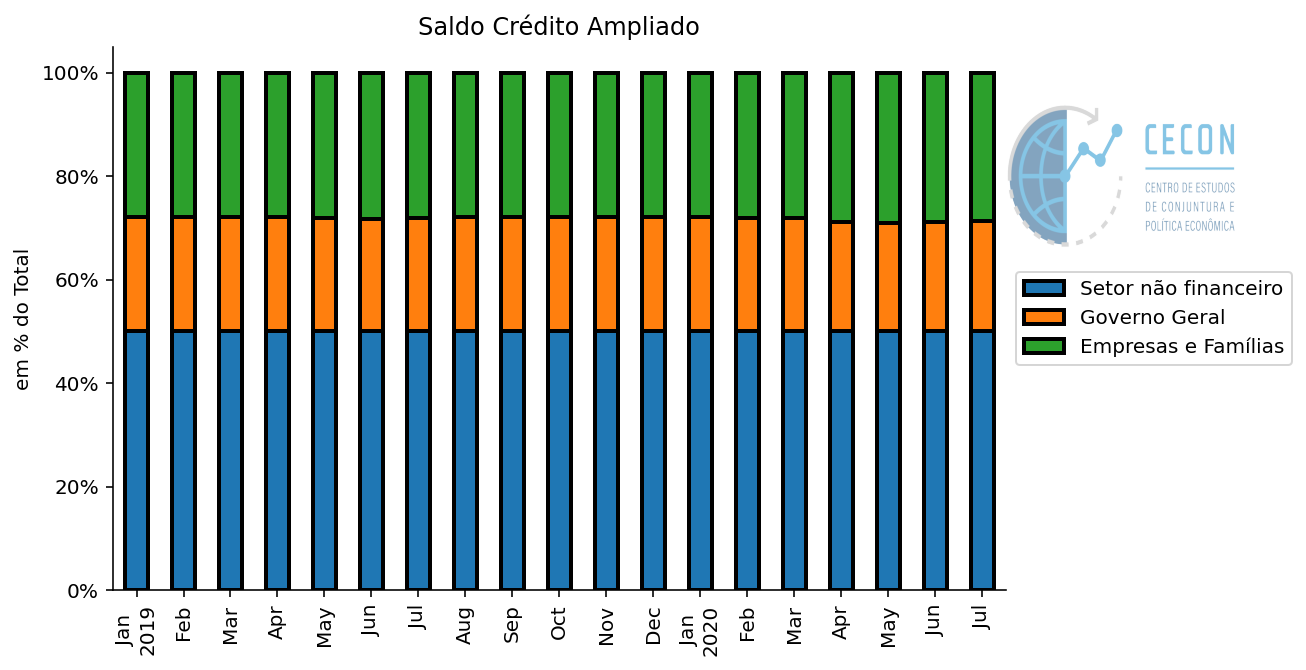
\includegraphics[width=.9\linewidth]{obipy-resources/62e383af79e91b63c7fc98dd7fb55b3c3ececcb9/fc25f4901d8007b52b37c8cc10e4620bc37873f2.png}
\end{center}

\begin{verbatim}
<Figure size 576x360 with 2 Axes>
\end{verbatim}


\begin{center}
\includegraphics[width=.9\linewidth]{obipy-resources/62e383af79e91b63c7fc98dd7fb55b3c3ececcb9/d787c0b50fa6cabeff88eb82b75849ce6f26ce84.png}
\end{center}


\begin{verbatim}
<Figure size 576x360 with 2 Axes>
\end{verbatim}


\begin{center}
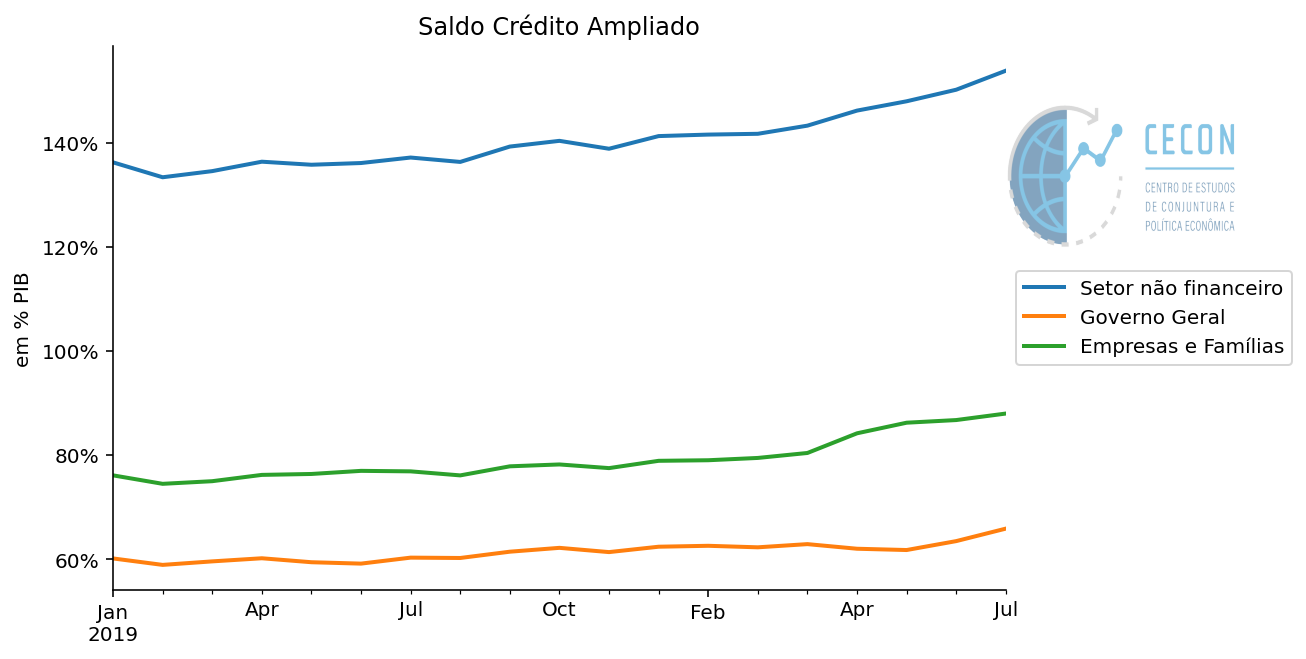
\includegraphics[width=.9\linewidth]{obipy-resources/62e383af79e91b63c7fc98dd7fb55b3c3ececcb9/71e2f6f170d1eae4c7e08b6bb69381e2fc6bfa43.png}
\end{center}

\item Crédito direcionado
\label{sec:orgfa4d88e}


\begin{verbatim}
<Figure size 576x360 with 2 Axes>
\end{verbatim}


\begin{center}
\includegraphics[width=.9\linewidth]{obipy-resources/62e383af79e91b63c7fc98dd7fb55b3c3ececcb9/ce90c1989329de9bd35e54499a49e998a229e167.png}
\end{center}

\begin{verbatim}
<Figure size 576x360 with 2 Axes>
\end{verbatim}


\begin{center}
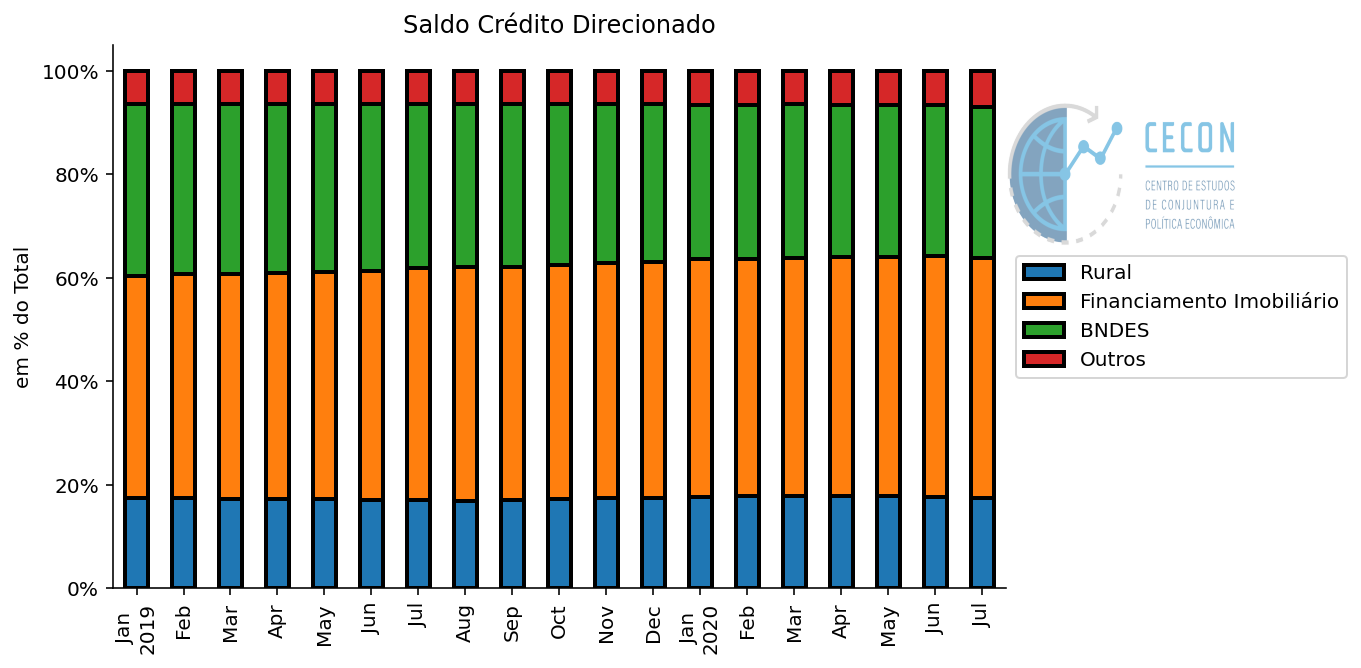
\includegraphics[width=.9\linewidth]{obipy-resources/62e383af79e91b63c7fc98dd7fb55b3c3ececcb9/9a2b55ba48387fe773ae71f452b084dae90c5a91.png}
\end{center}

\begin{verbatim}
<Figure size 576x360 with 2 Axes>
\end{verbatim}


\begin{center}
\includegraphics[width=.9\linewidth]{obipy-resources/62e383af79e91b63c7fc98dd7fb55b3c3ececcb9/120b087dfcc6ee8bca3227ec45868b7327bde212.png}
\end{center}
\end{enumerate}



\subsection{IBCBr}
\label{sec:org1afa811}

\emph{home/gpetrini}.local/lib/python3.8/site-packages/pandas\_datareader/compat/\_\_init\_\_.py:7: FutureWarning: pandas.util.testing is deprecated. Use the functions in the public API at pandas.testing instead.
  from pandas.util.testing import assert\_frame\_equal


\begin{verbatim}
<Figure size 576x360 with 2 Axes>
\end{verbatim}


\begin{center}
\includegraphics[width=.9\linewidth]{obipy-resources/62e383af79e91b63c7fc98dd7fb55b3c3ececcb9/51df5d2fc00ebe923cd476edd2384c8734922982.png}
\end{center}

\subsection{PIB (Contas Nacionais)}
\label{sec:org264744b}

Archive:  Tab\_Compl\_CNT.zip
  inflating: Tab\_Compl\_CNT\_1T20.xls  

\subsubsection{Trimestre Contra trimestre imediatamente anterior}
\label{sec:orgcfcbca0}

2019Q2    0.005406
2019Q3    0.004618
2019Q4    0.003655
2020Q1   -0.015394
Freq: Q-DEC, Name: PIB, dtype: float64

\begin{verbatim}
<Figure size 648x288 with 2 Axes>
\end{verbatim}


\begin{center}
\includegraphics[width=.9\linewidth]{obipy-resources/62e383af79e91b63c7fc98dd7fb55b3c3ececcb9/ccdd216b2d4ec7f442e7ee785f5dac79e8944214.png}
\end{center}

\begin{enumerate}
\item Agropecuária
\label{sec:org4a717ee}

\begin{verbatim}
<Figure size 648x288 with 2 Axes>
\end{verbatim}


\begin{center}
\includegraphics[width=.9\linewidth]{obipy-resources/62e383af79e91b63c7fc98dd7fb55b3c3ececcb9/a15942baa3e7c0f56f68b582422f779dbd39f086.png}
\end{center}

\item Indústria
\label{sec:org3c13022}

        Industria Extrativa  Industria de Transformacao  Eletricidade e agua  $\backslash$
2019Q2            -0.030796                    0.015653            -0.004612   
2019Q3             0.112907                   -0.008735            -0.013919   
2019Q4             0.006668                    0.001203             0.002735   
2020Q1            -0.032339                   -0.013738            -0.001341   

        Construcao  Total Industria  
2019Q2    0.019130         0.006188  
2019Q3    0.008864         0.007511  
2019Q4   -0.023357         0.000195  
2020Q1   -0.023948        -0.013793  

\begin{verbatim}
<Figure size 648x288 with 2 Axes>
\end{verbatim}


\begin{center}
\includegraphics[width=.9\linewidth]{obipy-resources/62e383af79e91b63c7fc98dd7fb55b3c3ececcb9/f8ca18e52f397fc50e1ff1d712275d10e5e066a0.png}
\end{center}


\item Serviços
\label{sec:org7fb67ce}

        Comercio  Transporte, armazenagem e correio  Informacao e comunicacao  $\backslash$
1996Q1       NaN                                NaN                       NaN   
1996Q2 -0.002371                          -0.028222                  0.015095   
1996Q3  0.025455                           0.036438                  0.021967   
1996Q4  0.015195                          -0.037310                 -0.001976   
1997Q1  0.002414                           0.040428                  0.011012   
\ldots{}          \ldots{}                                \ldots{}                       \ldots{}   
2019Q1  0.008961                          -0.002449                  0.011049   
2019Q2  0.006977                          -0.000455                  0.006743   
2019Q3  0.007517                          -0.003686                  0.010703   
2019Q4 -0.001857                           0.014547                  0.016215   
2020Q1 -0.007686                          -0.024192                 -0.019052   

        Atividades Financeiras  Atividades Imobiliarias  Outras atividades  $\backslash$
1996Q1                     NaN                      NaN                NaN   
1996Q2                0.001748                 0.006362          -0.005097   
1996Q3               -0.000033                 0.009057           0.002842   
1996Q4               -0.087280                -0.024478          -0.003531   
1997Q1                0.110854                 0.022929           0.014299   
\ldots{}                        \ldots{}                      \ldots{}                \ldots{}   
2019Q1                0.008045                 0.003100           0.001185   
2019Q2               -0.000677                 0.007525           0.003958   
2019Q3                0.013945                 0.002887           0.000598   
2019Q4                0.008249                 0.001962           0.008319   
2020Q1               -0.001175                 0.003511          -0.045997   

        ADM, defesa, etc  Total Servicos  
1996Q1               NaN             NaN  
1996Q2          0.008730        0.003606  
1996Q3          0.005202        0.016645  
1996Q4         -0.006725       -0.023475  
1997Q1         -0.000029        0.021750  
\ldots{}                  \ldots{}             \ldots{}  
2019Q1          0.004140        0.003870  
2019Q2         -0.002328        0.002439  
2019Q3         -0.007317        0.003180  
2019Q4          0.010108        0.006761  
2020Q1         -0.004807       -0.016362  

[97 rows x 8 columns]

\begin{verbatim}
<Figure size 648x288 with 2 Axes>
\end{verbatim}


\begin{center}
\includegraphics[width=.9\linewidth]{obipy-resources/62e383af79e91b63c7fc98dd7fb55b3c3ececcb9/c103d0839f7e2f5159d233a24313c78c17723e40.png}
\end{center}

\item Demanda
\label{sec:org7fdacab}

        Consumo das Familias  Consumo do Governo      FBCF  Exportacao  $\backslash$
2019Q2              0.004122           -0.002895  0.024859   -0.023292   
2019Q3              0.004586           -0.003876  0.017226   -0.023973   
2019Q4              0.004198            0.004176 -0.026872    0.022656   
2020Q1             -0.019856            0.002393  0.030928   -0.009145   

        Importacao       PIB  
2019Q2    0.014682  0.005406  
2019Q3    0.024805  0.004618  
2019Q4   -0.033197  0.003655  
2020Q1    0.028102 -0.015394  

\begin{verbatim}
<Figure size 648x288 with 2 Axes>
\end{verbatim}


\begin{center}
\includegraphics[width=.9\linewidth]{obipy-resources/62e383af79e91b63c7fc98dd7fb55b3c3ececcb9/02f06c0b594eedf9695736ccb4480c0d158223a9.png}
\end{center}

\item Oferta
\label{sec:org559dc62}


        Agropecuaria  Total Industria  Total Servicos       PIB
2019Q2      0.007891         0.006188        0.002439  0.005406
2019Q3      0.011709         0.007511        0.003180  0.004618
2019Q4     -0.004082         0.000195        0.006761  0.003655
2020Q1      0.005651        -0.013793       -0.016362 -0.015394

\begin{verbatim}
<Figure size 648x288 with 2 Axes>
\end{verbatim}


\begin{center}
\includegraphics[width=.9\linewidth]{obipy-resources/62e383af79e91b63c7fc98dd7fb55b3c3ececcb9/c8cf7a0405d1cf169bed23c97538f5064a093acc.png}
\end{center}
\end{enumerate}


\subsubsection{Contribuição para variação}
\label{sec:orgc9a0958}

\begin{enumerate}
\item Demanda
\label{sec:org493814d}

        Consumo das Familias  Consumo do Governo      FBCF  Exportacao  $\backslash$
2018Q2              0.000411            0.000829 -0.002023   -0.003944   
2018Q3              0.003452            0.000556  0.007673    0.008579   
2018Q4              0.001663           -0.002415 -0.000270    0.002493   
2019Q1              0.004940            0.001095 -0.002769   -0.005361   
2019Q2              0.002820           -0.000532  0.004298   -0.003278   
2019Q3              0.003134           -0.000706  0.003036   -0.003278   
2019Q4              0.002868            0.000755 -0.004795    0.003009   
2020Q1             -0.013574            0.000433  0.005351   -0.001238   

        Importacao  
2018Q2    0.003814  
2018Q3   -0.012351  
2018Q4    0.006794  
2019Q1    0.000665  
2019Q2   -0.002057  
2019Q3   -0.003507  
2019Q4    0.004788  
2020Q1   -0.003904  

\begin{verbatim}
<Figure size 432x288 with 1 Axes>
\end{verbatim}


\begin{center}
\includegraphics[width=.9\linewidth]{obipy-resources/62e383af79e91b63c7fc98dd7fb55b3c3ececcb9/0febddaa33fb2a03ea6f366eac4aad0fc9de4e3f.png}
\end{center}

\item Oferta
\label{sec:org0b0a149}

\emph{home/gpetrini}.local/lib/python3.8/site-packages/pandas/plotting/\_matplotlib/core.py:218: UserWarning: 'color' and 'colormap' cannot be used simultaneously. Using 'color'
  warnings.warn(
\emph{home/gpetrini}.local/lib/python3.8/site-packages/pandas/plotting/\_matplotlib/style.py:27: UserWarning: 'color' and 'colormap' cannot be used simultaneously. Using 'color'
  warnings.warn(
        Agropecuaria  Total Industria  Total Servicos
2018Q2      0.000223        -0.001063        0.001793
2018Q3      0.000821         0.000241        0.003313
2018Q4      0.000504        -0.000879        0.000476
2019Q1     -0.000773        -0.000027        0.002749
2019Q2      0.000624         0.001329        0.001736
2019Q3      0.000929         0.001616        0.002259
2019Q4     -0.000326         0.000042        0.004796
2020Q1      0.000447        -0.002961       -0.011628

\begin{verbatim}
<Figure size 648x288 with 2 Axes>
\end{verbatim}


\begin{center}
\includegraphics[width=.9\linewidth]{obipy-resources/62e383af79e91b63c7fc98dd7fb55b3c3ececcb9/7a30204ed9571e1428d4f79e14edbfb726d1b9cf.png}
\end{center}
\end{enumerate}

\subsubsection{Carregamento estatístico}
\label{sec:orgfb20c0d}



\section{Setor Externo}
\label{sec:org2a2e416}


\subsection{Balanço de Pagamentos}
\label{sec:orgbb60065}

\emph{home/gpetrini}.local/lib/python3.8/site-packages/pandas\_datareader/compat/\_\_init\_\_.py:7: FutureWarning: pandas.util.testing is deprecated. Use the functions in the public API at pandas.testing instead.
  from pandas.util.testing import assert\_frame\_equal


\subsubsection{Balança comercial}
\label{sec:org5472022}

\begin{verbatim}
<Figure size 576x360 with 2 Axes>
\end{verbatim}


\begin{center}
\includegraphics[width=.9\linewidth]{obipy-resources/62e383af79e91b63c7fc98dd7fb55b3c3ececcb9/1e0d8385dd451046cdb0d2ba3d5177a8c0b66b09.png}
\end{center}


\begin{verbatim}
<Figure size 576x360 with 2 Axes>
\end{verbatim}


\begin{center}
\includegraphics[width=.9\linewidth]{obipy-resources/62e383af79e91b63c7fc98dd7fb55b3c3ececcb9/5c8166f4bad84dd16ebefa571131cb142728daa5.png}
\end{center}


\begin{verbatim}
<Figure size 576x360 with 2 Axes>
\end{verbatim}


\begin{center}
\includegraphics[width=.9\linewidth]{obipy-resources/62e383af79e91b63c7fc98dd7fb55b3c3ececcb9/0c79e964de2ddd1cb6e026cbcf8475b6f5849d98.png}
\end{center}


\subsubsection{Conta corrente (\%PIB)}
\label{sec:org51e8e44}

\begin{verbatim}
<Figure size 576x360 with 2 Axes>
\end{verbatim}


\begin{center}
\includegraphics[width=.9\linewidth]{obipy-resources/62e383af79e91b63c7fc98dd7fb55b3c3ececcb9/1c5d34e0d8ec55b286fb4de024d0b7b11b8bcf58.png}
\end{center}

\subsubsection{Balança Comercial por país (mensal)}
\label{sec:org0a67251}

\begin{verbatim}
<Figure size 576x360 with 2 Axes>
\end{verbatim}


\begin{center}
\includegraphics[width=.9\linewidth]{obipy-resources/62e383af79e91b63c7fc98dd7fb55b3c3ececcb9/c3ff075133f390045c0fb620ae17d0d8ae93f0b8.png}
\end{center}


\begin{verbatim}
<Figure size 576x360 with 2 Axes>
\end{verbatim}


\begin{center}
\includegraphics[width=.9\linewidth]{obipy-resources/62e383af79e91b63c7fc98dd7fb55b3c3ececcb9/94e3a318f5fa3b548791774e379fcc93c0ac6151.png}
\end{center}

\begin{enumerate}
\item Importações
\label{sec:org719412b}

\begin{verbatim}
<Figure size 576x360 with 2 Axes>
\end{verbatim}


\begin{center}
\includegraphics[width=.9\linewidth]{obipy-resources/62e383af79e91b63c7fc98dd7fb55b3c3ececcb9/418cb4f4d4375891918713f399f1fd90e9c5c223.png}
\end{center}


\begin{verbatim}
<Figure size 576x360 with 2 Axes>
\end{verbatim}


\begin{center}
\includegraphics[width=.9\linewidth]{obipy-resources/62e383af79e91b63c7fc98dd7fb55b3c3ececcb9/5deabc9a2c1ef0035dab475172a88f0cbcbb7efa.png}
\end{center}
\end{enumerate}


\subsubsection{Saldo Comercial}
\label{sec:org67f0ae7}

\begin{verbatim}
<Figure size 576x360 with 2 Axes>
\end{verbatim}


\begin{center}
\includegraphics[width=.9\linewidth]{obipy-resources/62e383af79e91b63c7fc98dd7fb55b3c3ececcb9/45699a516d97feebeb7f7e04293a5e946ff61c4c.png}
\end{center}


\begin{verbatim}
<Figure size 576x360 with 2 Axes>
\end{verbatim}


\begin{center}
\includegraphics[width=.9\linewidth]{obipy-resources/62e383af79e91b63c7fc98dd7fb55b3c3ececcb9/21bc45cb0da9893e5fef8023e5101cfef69cdbcb.png}
\end{center}

\subsection{China}
\label{sec:orgd808720}

\emph{home/gpetrini}.local/lib/python3.8/site-packages/pandas\_datareader/compat/\_\_init\_\_.py:7: FutureWarning: pandas.util.testing is deprecated. Use the functions in the public API at pandas.testing instead.
  from pandas.util.testing import assert\_frame\_equal


\begin{verbatim}
<Figure size 576x360 with 2 Axes>
\end{verbatim}


\begin{center}
\includegraphics[width=.9\linewidth]{obipy-resources/62e383af79e91b63c7fc98dd7fb55b3c3ececcb9/c74b91ccd85342cb8d46bc2adf505f782f53168c.png}
\end{center}

\begin{verbatim}
<Figure size 576x360 with 2 Axes>
\end{verbatim}


\begin{center}
\includegraphics[width=.9\linewidth]{obipy-resources/62e383af79e91b63c7fc98dd7fb55b3c3ececcb9/c8d7570e3a7e977e5c224522a2254ee152c9b730.png}
\end{center}



\section{Índices de atividade setoriais}
\label{sec:org5f57953}

\emph{home/gpetrini}.local/lib/python3.8/site-packages/pandas\_datareader/compat/\_\_init\_\_.py:7: FutureWarning: pandas.util.testing is deprecated. Use the functions in the public API at pandas.testing instead.
  from pandas.util.testing import assert\_frame\_equal


\subsection{Pesquisa Industrial Mensal (PIM)}
\label{sec:orgd24c7b9}

\begin{verbatim}
<Figure size 576x360 with 2 Axes>
\end{verbatim}


\begin{center}
\includegraphics[width=.9\linewidth]{obipy-resources/62e383af79e91b63c7fc98dd7fb55b3c3ececcb9/d717735925d5d1c2f0e440c2e6c066139a4df3f4.png}
\end{center}


\subsection{Pesquisa Mensal do Comércio (PMC)}
\label{sec:orgddcfd29}

\begin{verbatim}
<Figure size 576x360 with 2 Axes>
\end{verbatim}


\begin{center}
\includegraphics[width=.9\linewidth]{obipy-resources/62e383af79e91b63c7fc98dd7fb55b3c3ececcb9/b534b097cb3117627d0996f21cbf6e828f0327f9.png}
\end{center}


\subsection{Pesquisa Mensal de Serviços (PMS)}
\label{sec:org3cdd0d6}

\begin{verbatim}
<Figure size 576x360 with 2 Axes>
\end{verbatim}


\begin{center}
\includegraphics[width=.9\linewidth]{obipy-resources/62e383af79e91b63c7fc98dd7fb55b3c3ececcb9/d4ec944fdf0da4f21e1332a03a296d7dcb2c7cd7.png}
\end{center}

\section{Emprego}
\label{sec:org09b3b2c}

\emph{home/gpetrini}.local/lib/python3.8/site-packages/pandas\_datareader/compat/\_\_init\_\_.py:7: FutureWarning: pandas.util.testing is deprecated. Use the functions in the public API at pandas.testing instead.
  from pandas.util.testing import assert\_frame\_equal


\subsection{Taxa de desocupação}
\label{sec:orge443466}

\begin{verbatim}
<Figure size 576x360 with 2 Axes>
\end{verbatim}


\begin{center}
\includegraphics[width=.9\linewidth]{obipy-resources/62e383af79e91b63c7fc98dd7fb55b3c3ececcb9/3e66e5d7c90078e7768d9ebdeb4b854b64554dc0.png}
\end{center}


\subsection{Massa de renda}
\label{sec:org3069e89}

\begin{verbatim}
<Figure size 576x360 with 2 Axes>
\end{verbatim}


\begin{center}
\includegraphics[width=.9\linewidth]{obipy-resources/62e383af79e91b63c7fc98dd7fb55b3c3ececcb9/12f387dcc997a1e058ff9556ac8d26b3954897ca.png}
\end{center}


\subsection{Desalentados e subocupados}
\label{sec:org4dc0dc9}

\begin{verbatim}
<Figure size 576x360 with 2 Axes>
\end{verbatim}


\begin{center}
\includegraphics[width=.9\linewidth]{obipy-resources/62e383af79e91b63c7fc98dd7fb55b3c3ececcb9/f32bc3ff2934cd6e25217103bf3cc674577be1da.png}
\end{center}

\subsection{Rendimento habitual médio por atividade}
\label{sec:orgab0c5fd}


\begin{verbatim}
<Figure size 576x360 with 2 Axes>
\end{verbatim}


\begin{center}
\includegraphics[width=.9\linewidth]{obipy-resources/62e383af79e91b63c7fc98dd7fb55b3c3ececcb9/7aaad0ee1869882066c6cd4e35e4b0fdd2c933bc.png}
\end{center}

\subsection{População ocupada por atividade}
\label{sec:orgb64f5d0}

\begin{verbatim}
<Figure size 576x360 with 2 Axes>
\end{verbatim}


\begin{center}
\includegraphics[width=.9\linewidth]{obipy-resources/62e383af79e91b63c7fc98dd7fb55b3c3ececcb9/18ae86fa0395bd8722bf758ae72aaa47ff7d9d15.png}
\end{center}



\subsection{Taxa de ocupação}
\label{sec:org278f013}

\begin{verbatim}
<Figure size 576x360 with 2 Axes>
\end{verbatim}


\begin{center}
\includegraphics[width=.9\linewidth]{obipy-resources/62e383af79e91b63c7fc98dd7fb55b3c3ececcb9/e57bbb759924a9cb6416ba0e9df75b2ce0d735dd.png}
\end{center}


\begin{verbatim}
<Figure size 576x360 with 2 Axes>
\end{verbatim}


\begin{center}
\includegraphics[width=.9\linewidth]{obipy-resources/62e383af79e91b63c7fc98dd7fb55b3c3ececcb9/e61012cac93df689012036ff07e2747e523e77b1.png}
\end{center}
\end{document}
